\subsection{Module type B, ``DESY Module''}
\label{chap:TPC_sec:DESY_gems}
Most recent update: 2020-05-14 \\
Contact person: Ties Behnke (email: ties.behnke@desy.de)\\

The goal of module type B is a maximal coverage of the end plate with minimal dead area and a low material budget. It relies on thin ceramic frames to support the GEM foils on top of the readout plane \cite{Hallermann:2010zz,2012arXiv1202.6510D}, see figure \ref{fig:moduleAssembled}. The high stiffness of the ceramic frame allows the construction of very thin frames, which in turn minimise the dead areas of the module. With the current design only $\sim5\%$ of the active area is taken by the support structure and gaps between modules, the rest is sensitive area. The design of the system allows the simple stacking of GEM foils to build up compact, light weight self supporting multi-GEM modules. The development of this module type is led by DESY.

\begin{figure}
\begin{subfigure}[b]{0.52\textwidth}
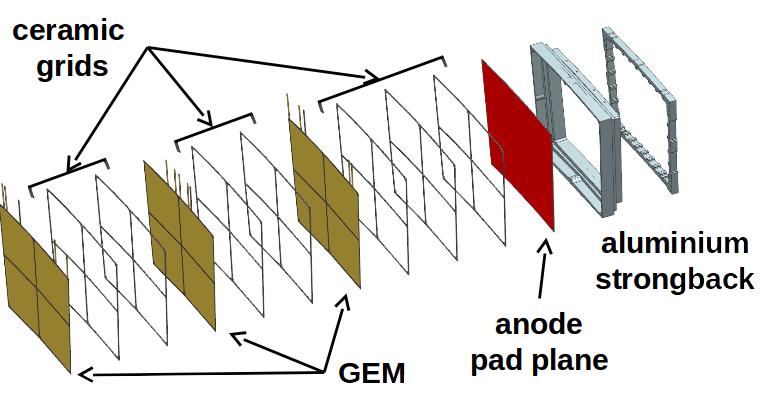
\includegraphics[width=\textwidth]{Tracker/TPC_Bonn/plots/TPC-DG_GemModule_Explosion.png}
\caption{}
\label{sfig:moduleExp}
\end{subfigure}
\hfill
\begin{subfigure}[b]{0.44\textwidth}
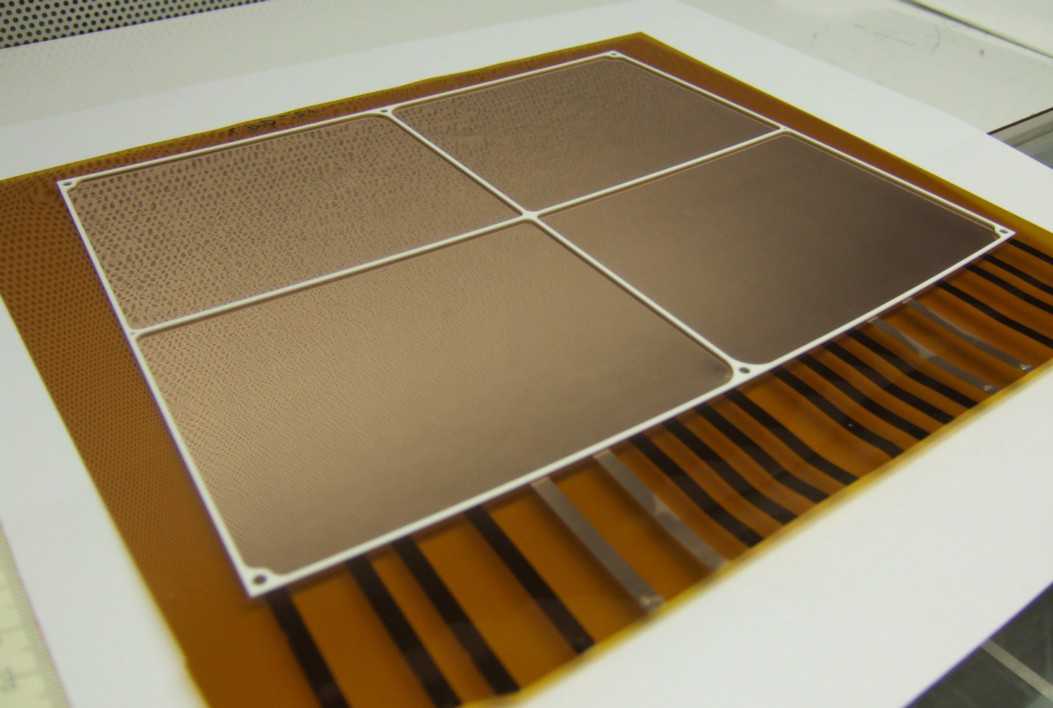
\includegraphics[width=\textwidth]{Tracker/TPC_Bonn/plots/TPC-DG_GemGrid.png}
\caption{}
\label{sfig:moduleGEM}
\end{subfigure}
\caption [Readout Module GEM]{\small \protect\subref{sfig:moduleExp})~Exploded view of one module showing the sequence of GEM foils and ceramic frames. \protect\subref{sfig:moduleGEM})~GEM foil with ceramic frame support used in the construction of the modules (used with permission from the LCTPC Collaboration as authors of the article ``A time projection chamber with GEM-based readout'', Nuclear Instruments and Methods in Physics Research A 856 (2017) 109–118, Elsevier, copyright 2016~\cite{FMueller2017}).}
\label{fig:moduleAssembled}
\end{figure}

\subsubsection{Recent Milestones}
Over the last years, several test-beam campaigns took place and exposed three GEM based modules to an electron beam. Extensive data sets were collected with and without magnetic field, at different working points, and at different angles between the TPC and the beam.

\paragraph{Distortion Correction}
Data taken in a 2013 beam test was used in a global attempt to determine and correct field distortions. 
The Millepede II \cite{Blobel20065,millepedeWiki} program was used to perform this global fit. 
The results indicate that distortions as large as several millimetres can be well corrected, see figure \ref{fig:1Tdistort}. 
All results of this beam-test campaign can be found in~\cite{FMueller2017} and~\cite{Mueller:301339}.

\begin{figure}
\centering
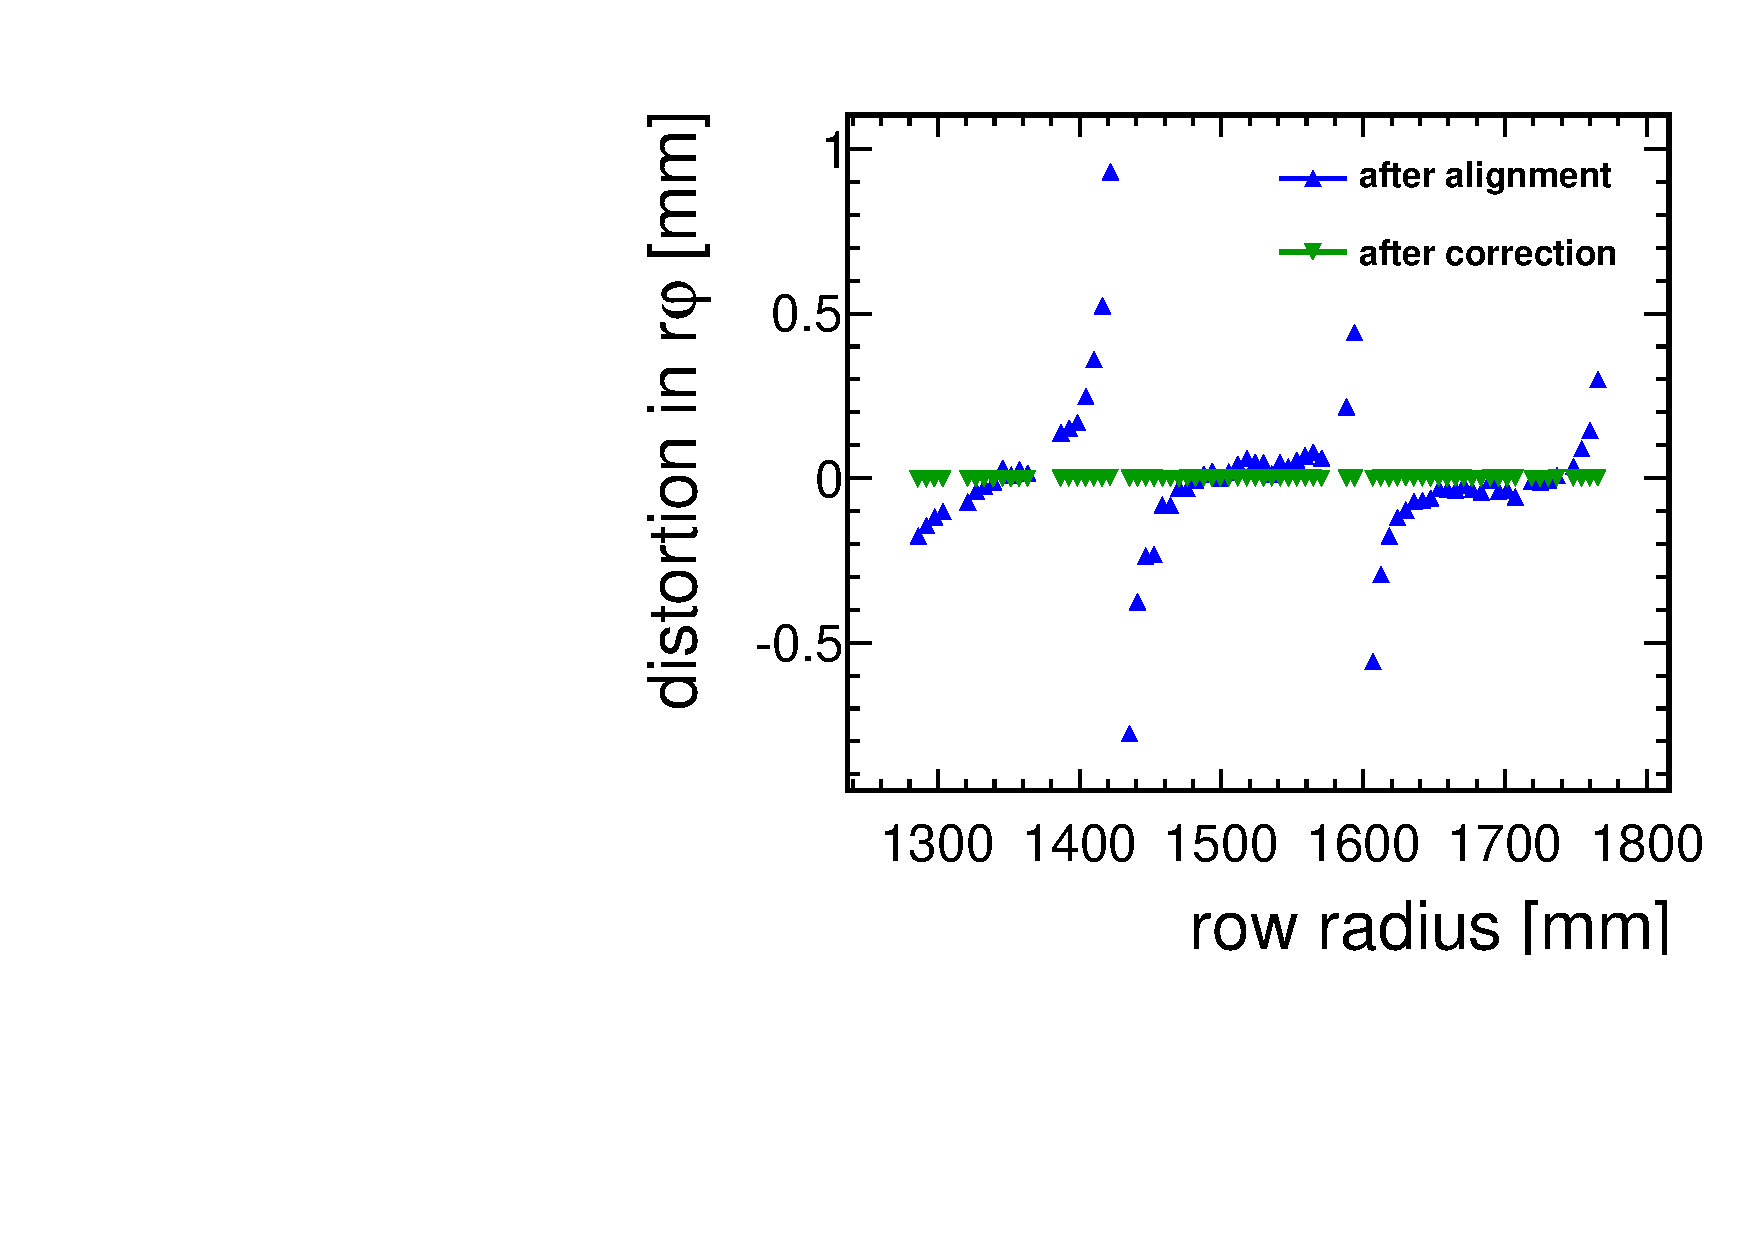
\includegraphics[width=0.48\textwidth]{Tracker/TPC_Bonn/plots/TPC-DG_distortionAlignmentPaper1Tdistcor.pdf}
\caption{\small~Alignment and distortion correction: mean hit position in $r\varphi$ with respect to the track position at \SI{1}{T} versus pad row radius. In blue after alignment correction, in green after distortion correction.}
\label{fig:1Tdistort}
\end{figure}

The field homogeneity was in addition studied in dedicated laser runs \cite{Zenker:2014qra}. A UV laser illuminates the cathode plane in the TPC, on which dots are placed made from a material with a small work function. The laser light extracts electrons at the position of the dots. These electrons are then drifted towards the anode, and are measured. From the dislocations of the dots relative to the known position on the cathode, the integrated effect of field distortions in the TPC volume can be measured.

\paragraph{Optimisation of Module Design and Production}

In 2016, a new generation GEM readout modules was produced. Here, the high voltage design and the production techniques were in the focus. 
The high voltage design of the single GEM foils was optimised in two ways. 
First, the hole pattern was revised so that at all places a minimum distance of \SI{0.5}{\mm} is ensured between a GEM hole and the ceramic frame or the glue, respectively.  
This was done since studies showed that glue spilling into the GEM holes tend to cause a decreased high voltage stability of the GEM. 
Second, instead of using a common high voltage layout for all GEM layers, adjusted layouts of the electrodes was implemented depending on the position of the GEM in the stack. 
In this way, cutting of the unused electrodes in a layer leading to sharp edges with high field areas were avoided.

Dedicated tooling was developed to stretch the GEM foils uniformly and glue them controlled and reproducible on the ceramic grids, see figure \ref{fig:gemstretch}. 
With this tooling, the quality of the GEM mounting, especially regarding the resulting flatness of the foils, could be improved significantly in comparison to the previous production, see figure \ref{sfig:GEMheight}.
In addition, the tool ensures for the correct alignment of the ceramic frame to the GEM foil and and allows for the reproducibility of the achieved high quality.
The improved flatness, with an RMS of only \SI{0.096}{\mm} of the height distribution, leads to a much improved gain uniformity. 
Over the module area, the deviation from the normalised gain is now only 0.036 as shown in figure \ref{sfig:GEMeffGain}.

\begin{figure}
    \centering
    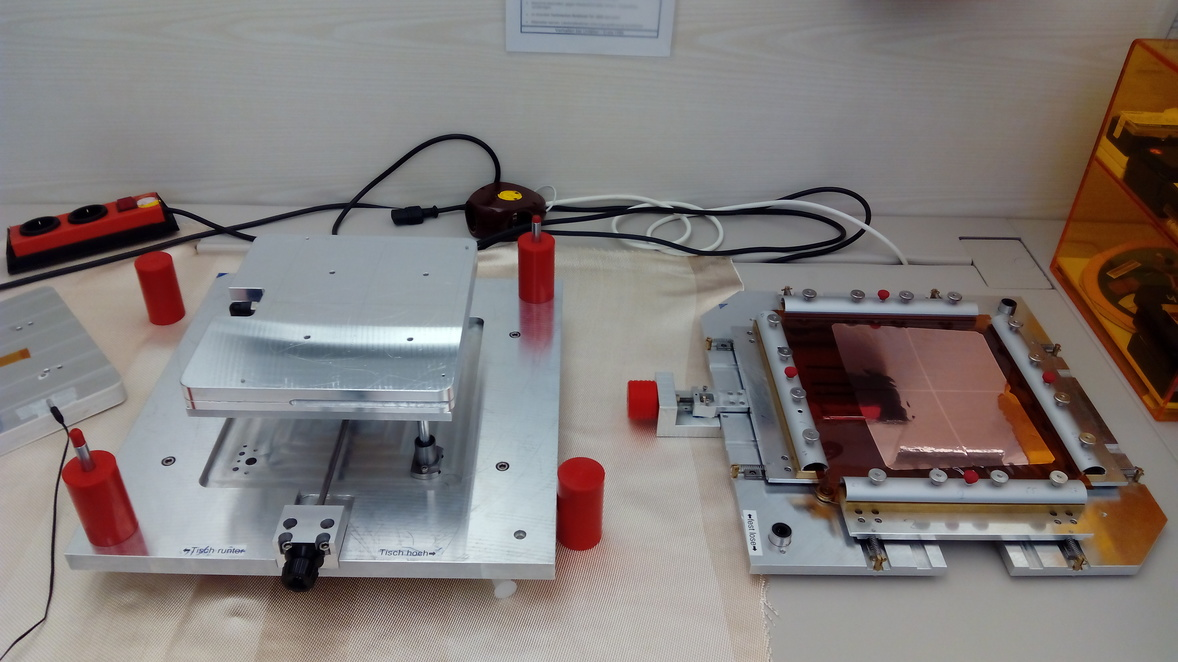
\includegraphics[height=0.4\textwidth]{Tracker/TPC_Bonn/plots/TPC-DG_stretching_tool.jpg}
    \caption{Picture of the stretching tool. The left part positions the ceramic frame, holding it with a vacuum system. The right part tensions the GEM foil and is applied to the bottom part after the glue has been deposited on the ceramic frame by a robotized dispenser.}
    \label{fig:gemstretch}
\end{figure}

\begin{figure}
\begin{subfigure}[b]{0.5\textwidth}
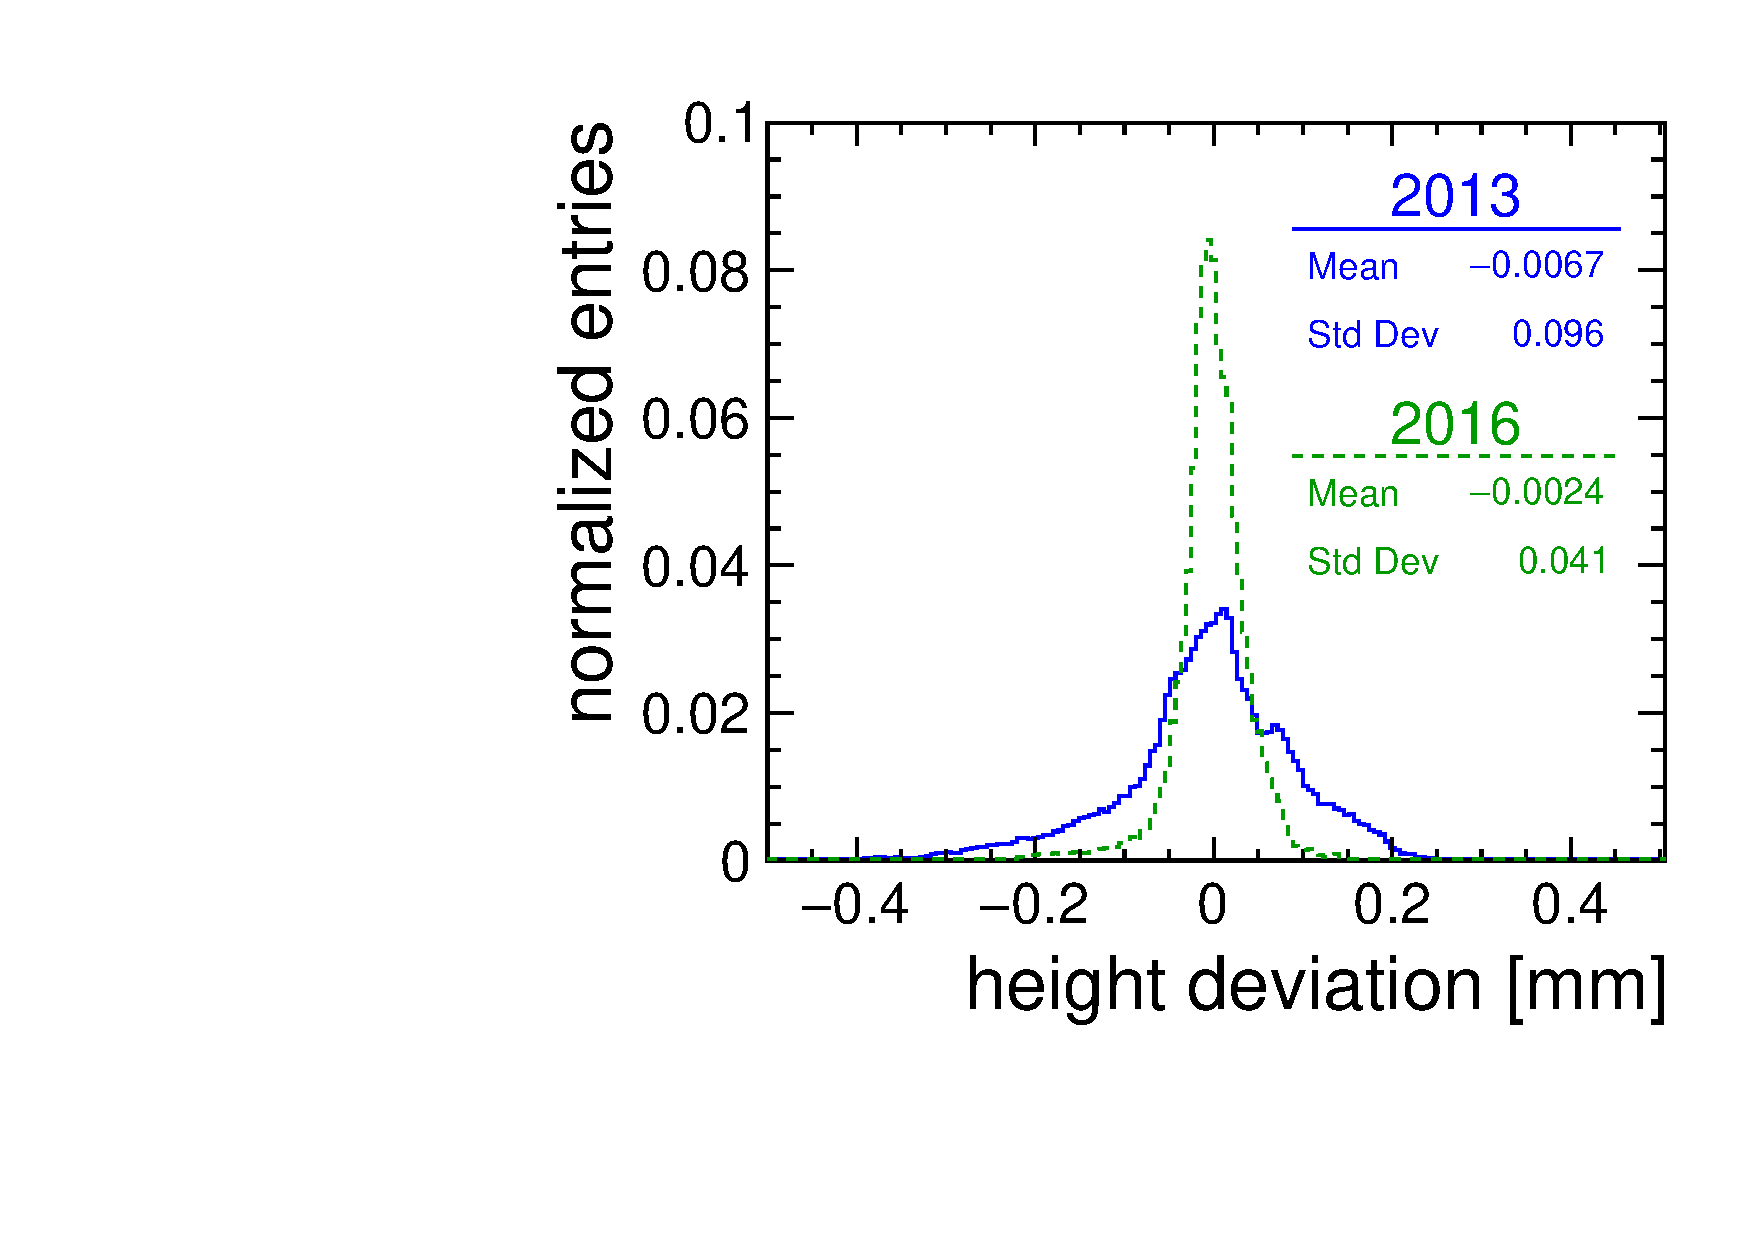
\includegraphics[width=\textwidth]{Tracker/TPC_Bonn/plots/TPC-DG_GEMHeightDistAll2013_2016comb_intnorm.pdf}
\caption{Measured GEM height deviations.}
\label{sfig:GEMheight}
\end{subfigure}%
\begin{subfigure}[b]{0.5\textwidth}
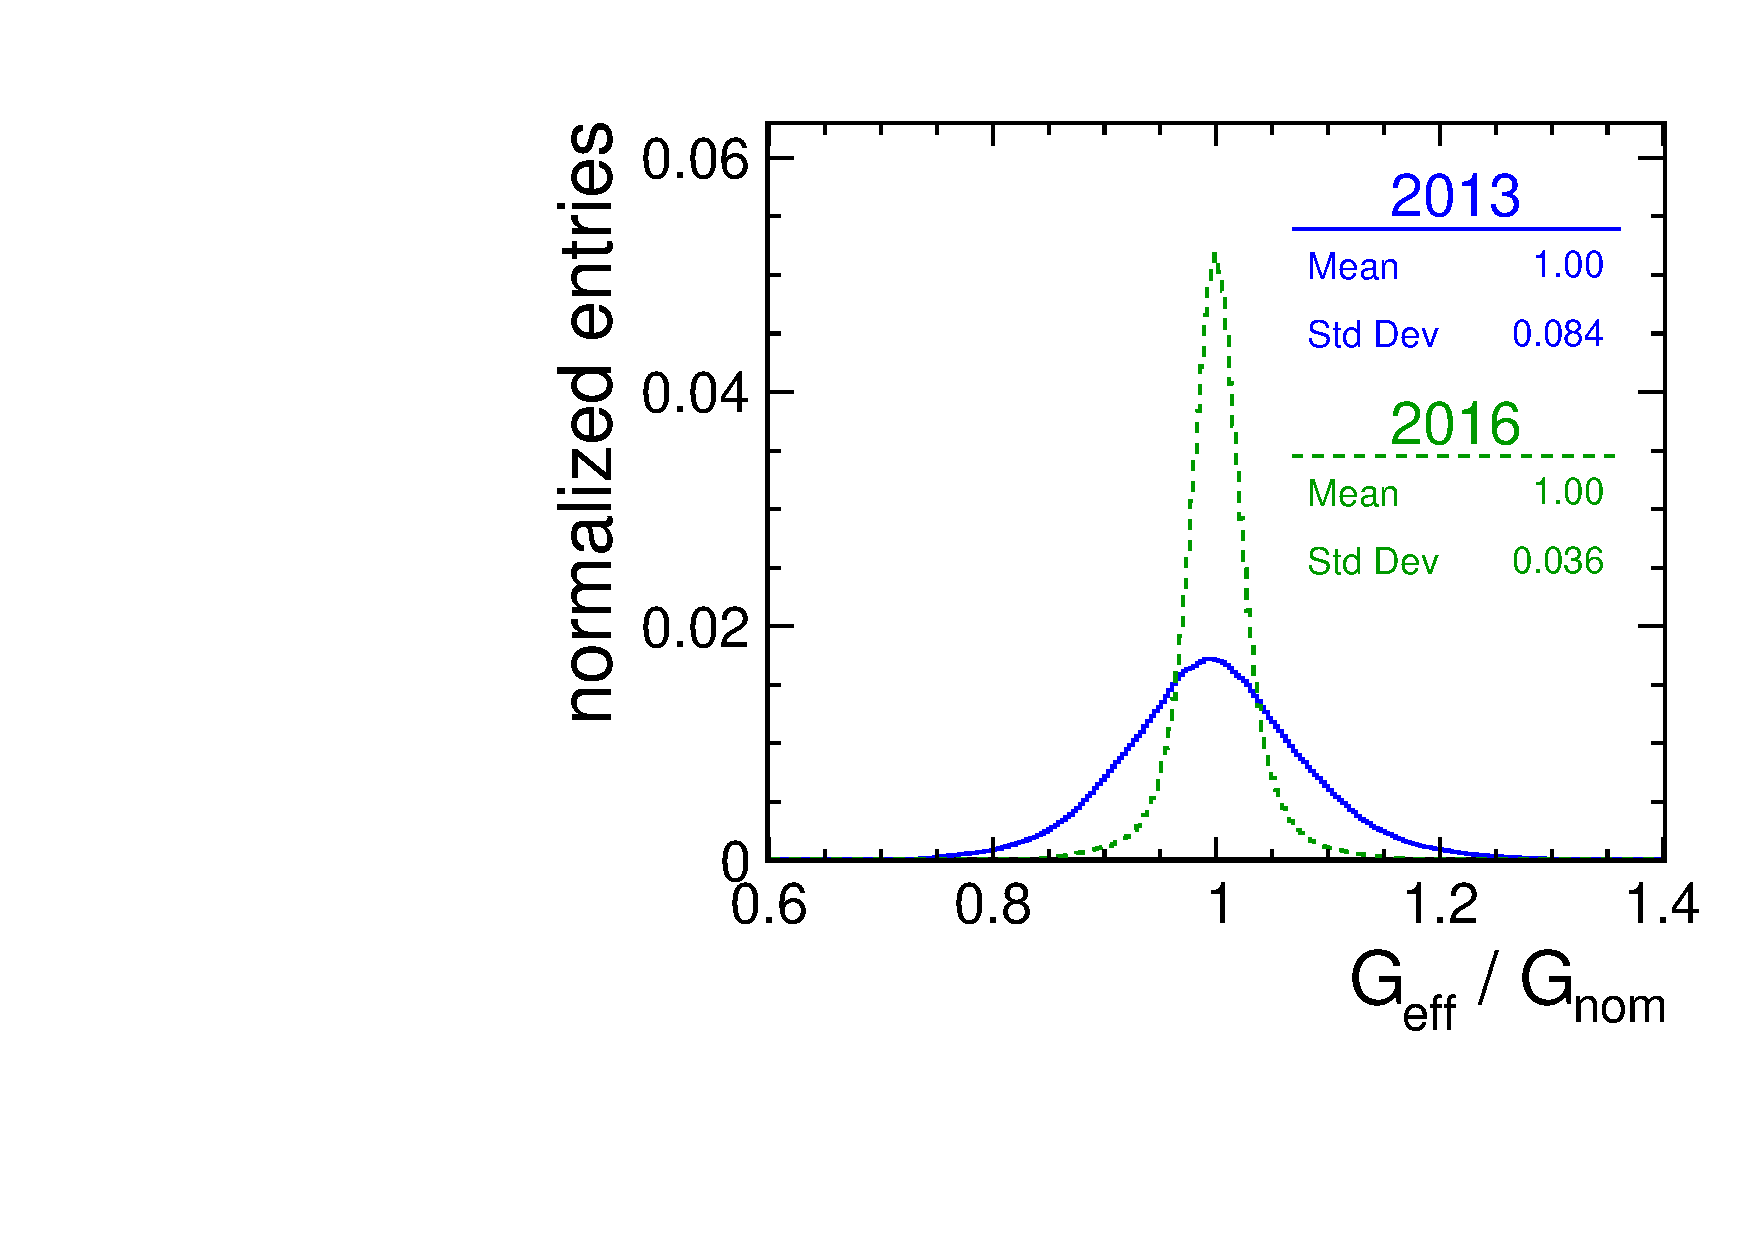
\includegraphics[width=\textwidth]{Tracker/TPC_Bonn/plots/TPC-DG_effectiveGainDistributionAll2013_2016comb_intnorm.pdf}
\caption{Calculated module gain deviations.}
\label{sfig:GEMeffGain}
\end{subfigure}
\caption{\protect\subref*{sfig:GEMheight})~Distribution of the measured height deviation for the old (2013) and new (2016) GEM modules and \protect\subref*{sfig:GEMeffGain})~the corresponding effective gain of the system, normalized to the nominal gain for perfectly flat GEMs.}
\label{fig:GEMheight}
\end{figure}

\paragraph{Point Resolution}

Based on an extensive beam-test campaign end of 2016, the performance of the new modules has been analysed in comparison to the previous module generation.
Figure \ref{fig:pointresolution} shows the comparison of the point resolution in $r\varphi$ and in the $z$ direction over the drift length of the prototype. The reproducibility of the results is clearly visible.

\begin{figure}
\begin{subfigure}[b]{0.48\textwidth}
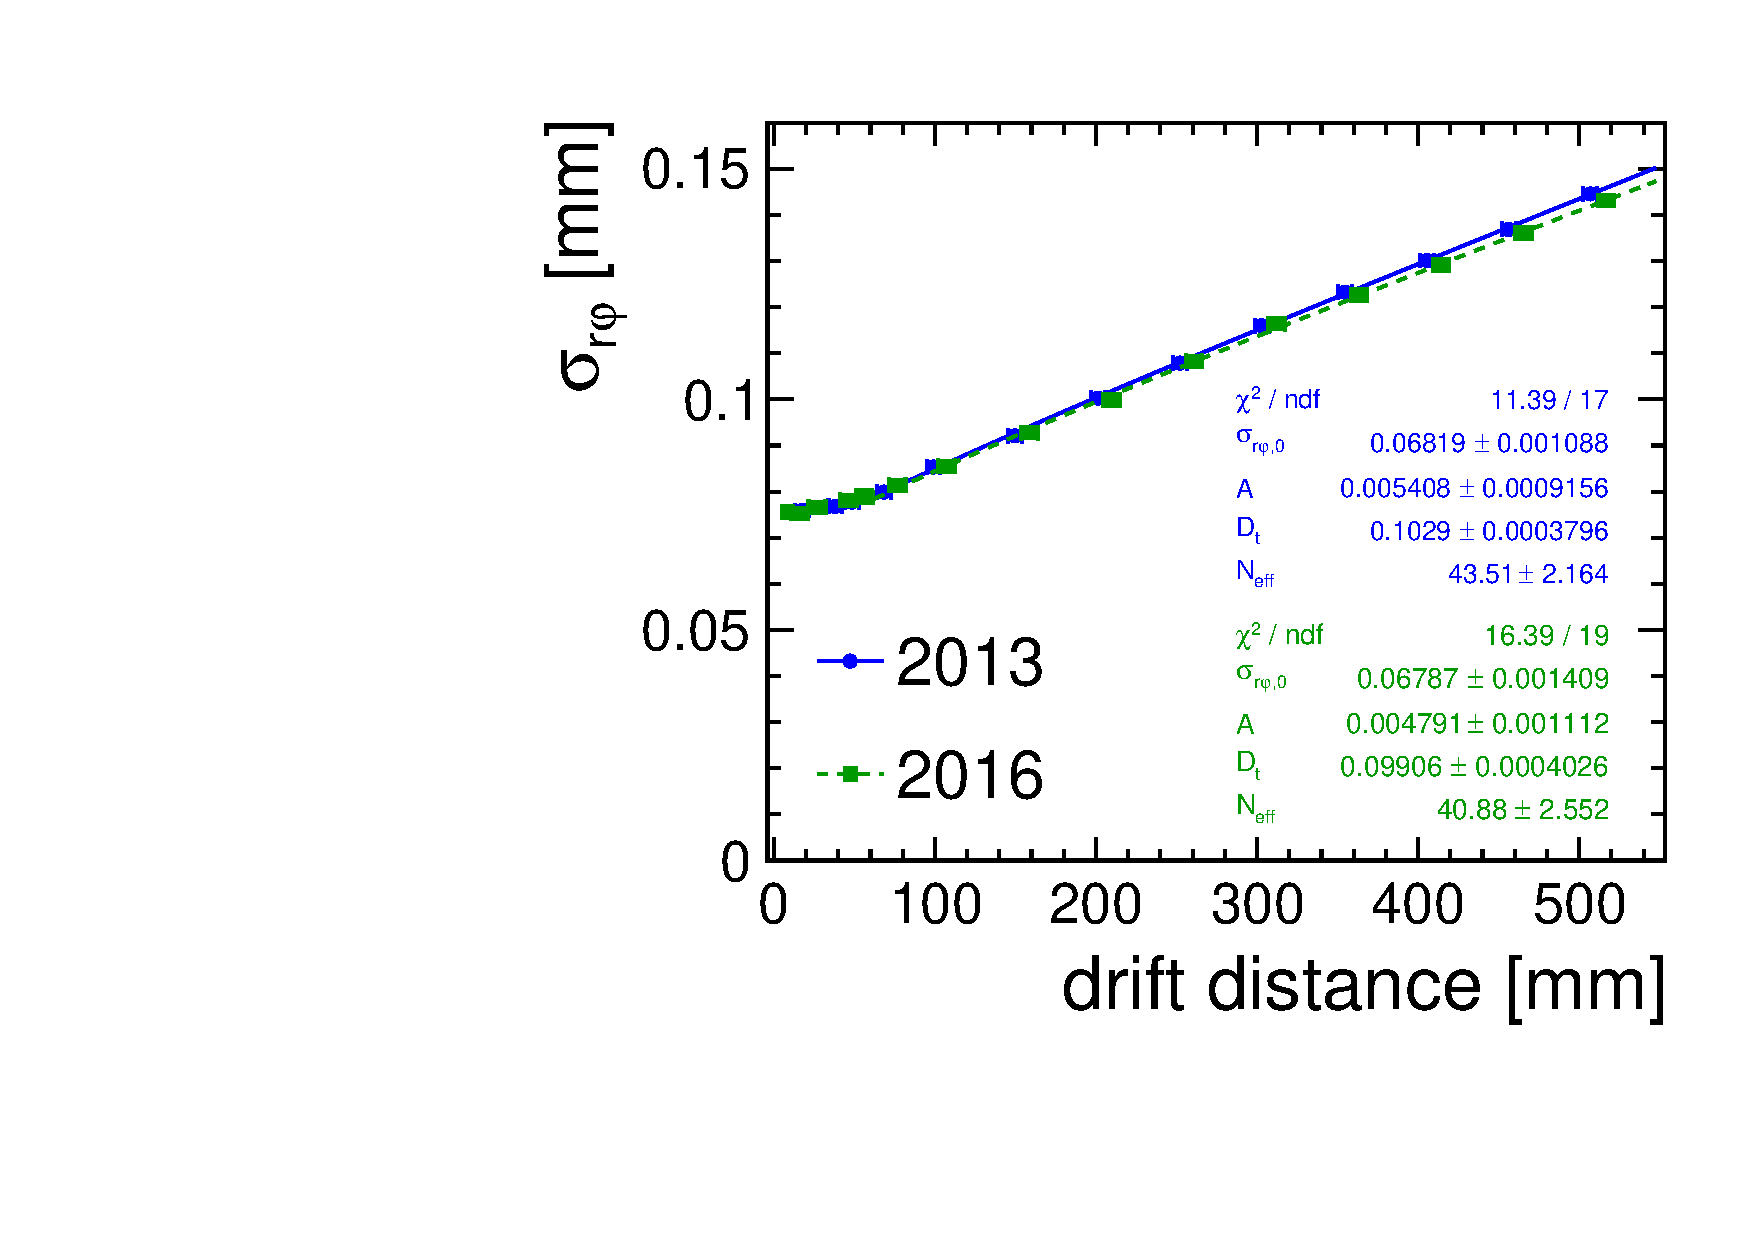
\includegraphics[width=\textwidth]{Tracker/TPC_Bonn/plots/TPC-DG_rphiResolution_combi_fit_global.pdf}
\caption{$r\varphi$-resolution.}
\label{sfig:pres_13-16_rphi}
\end{subfigure}
\hfill
\begin{subfigure}[b]{0.48\textwidth}
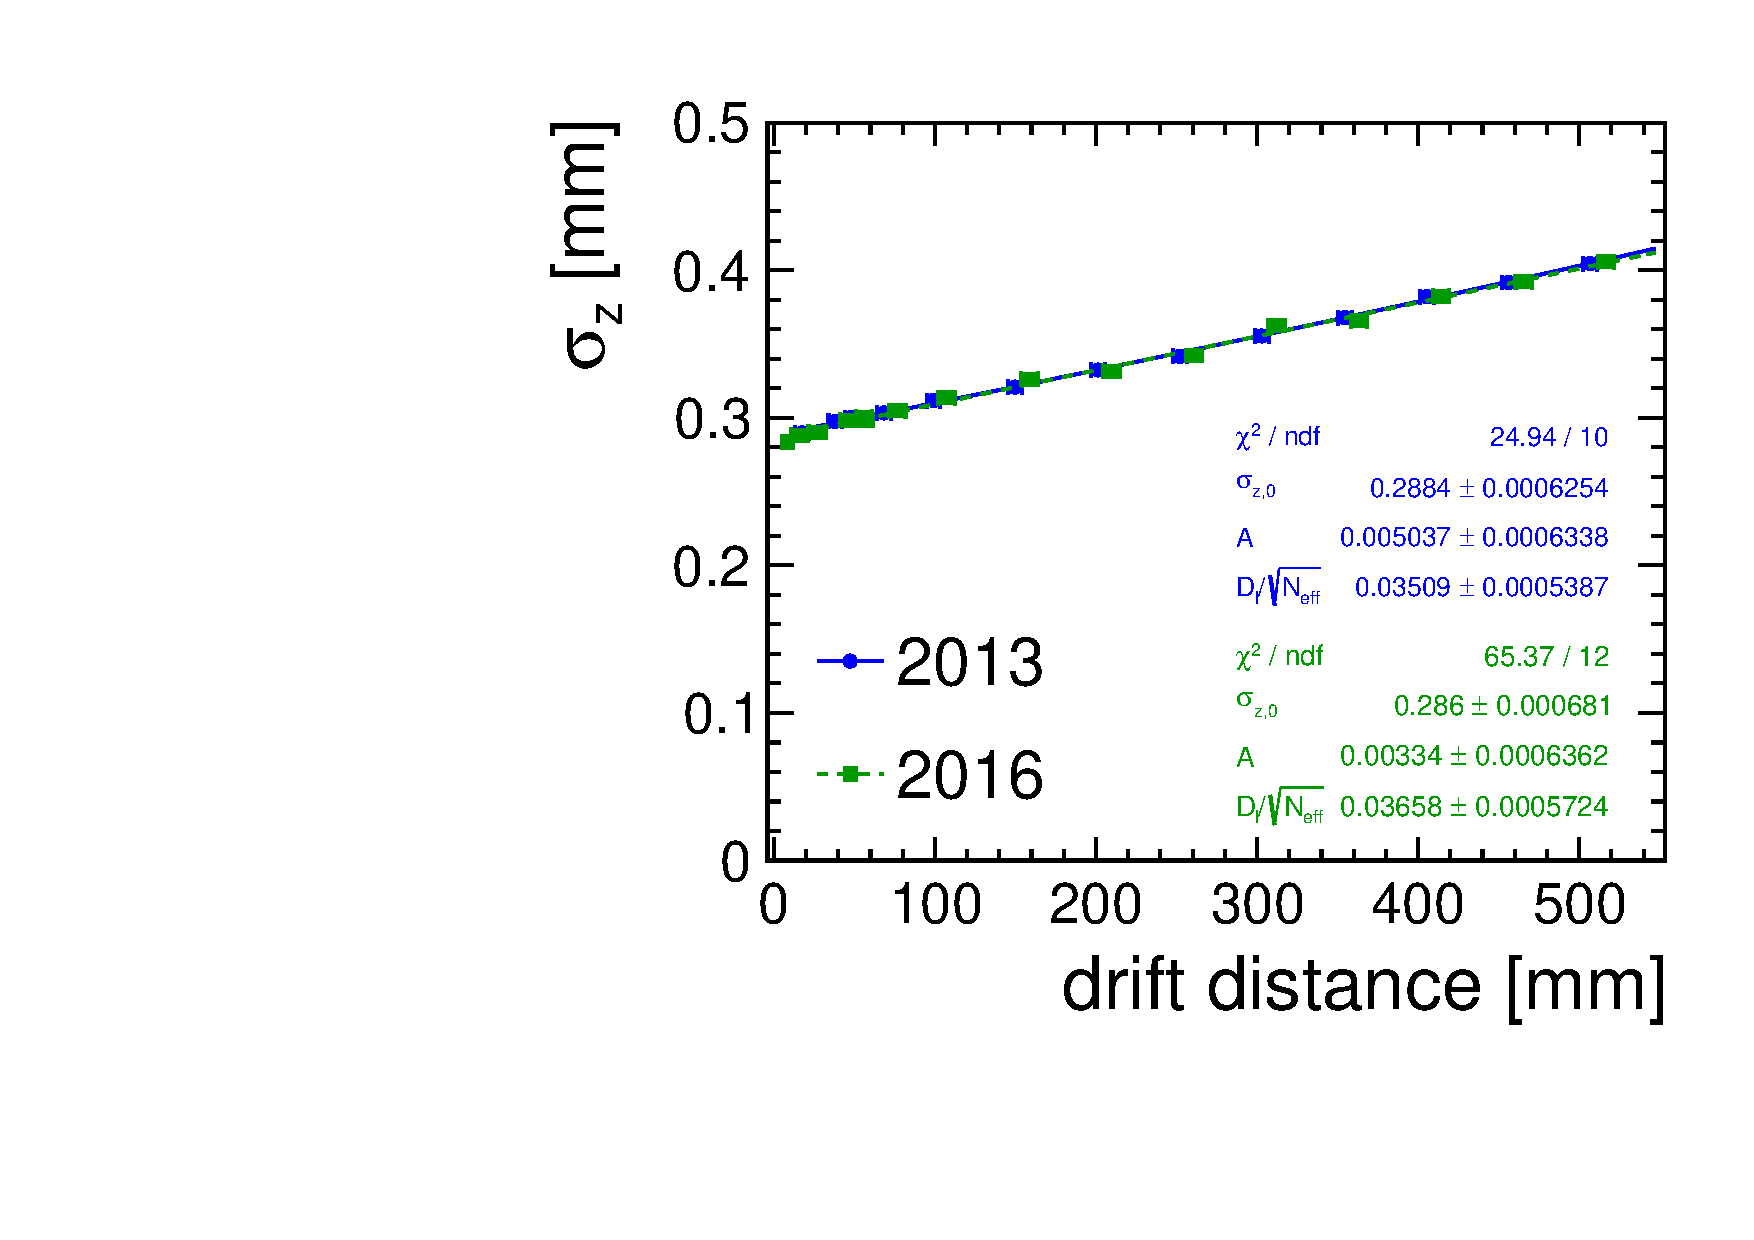
\includegraphics[width=\textwidth]{Tracker/TPC_Bonn/plots/TPC-DG_zResolution_combi_fit.pdf}
\caption{$z$-resolution.}
\label{sfig:pres_13-16_z}
\end{subfigure}
\caption{Comparison of the measured point resolution for current (2016) and previous (2013) module generation in \protect\subref*{sfig:pres_13-16_rphi})~$r\varphi$ and \protect\subref*{sfig:pres_13-16_z})~$z$ direction, both plotted versus the drift length.
  The lines represent fits of the resolution dependence on the drift length $z$ including electron loss due to attachment.
}
\label{fig:pointresolution}
\end{figure}

Based on these results, an extrapolation to the parameters of the ILD TPC has been done, once using the attachment rate determined at the beam test and once with an attachment rate set to zero. 
The results are shown in figure \ref{fig:resextrapol}. 
With an attachment rate of zero, the resolution requirement at the ILD experiment can be achieved. 
TPCs in running experiments as T2K or ALICE demonstrated that the necessary control of the gas conditions is possible.

\begin{figure}
    \centering
    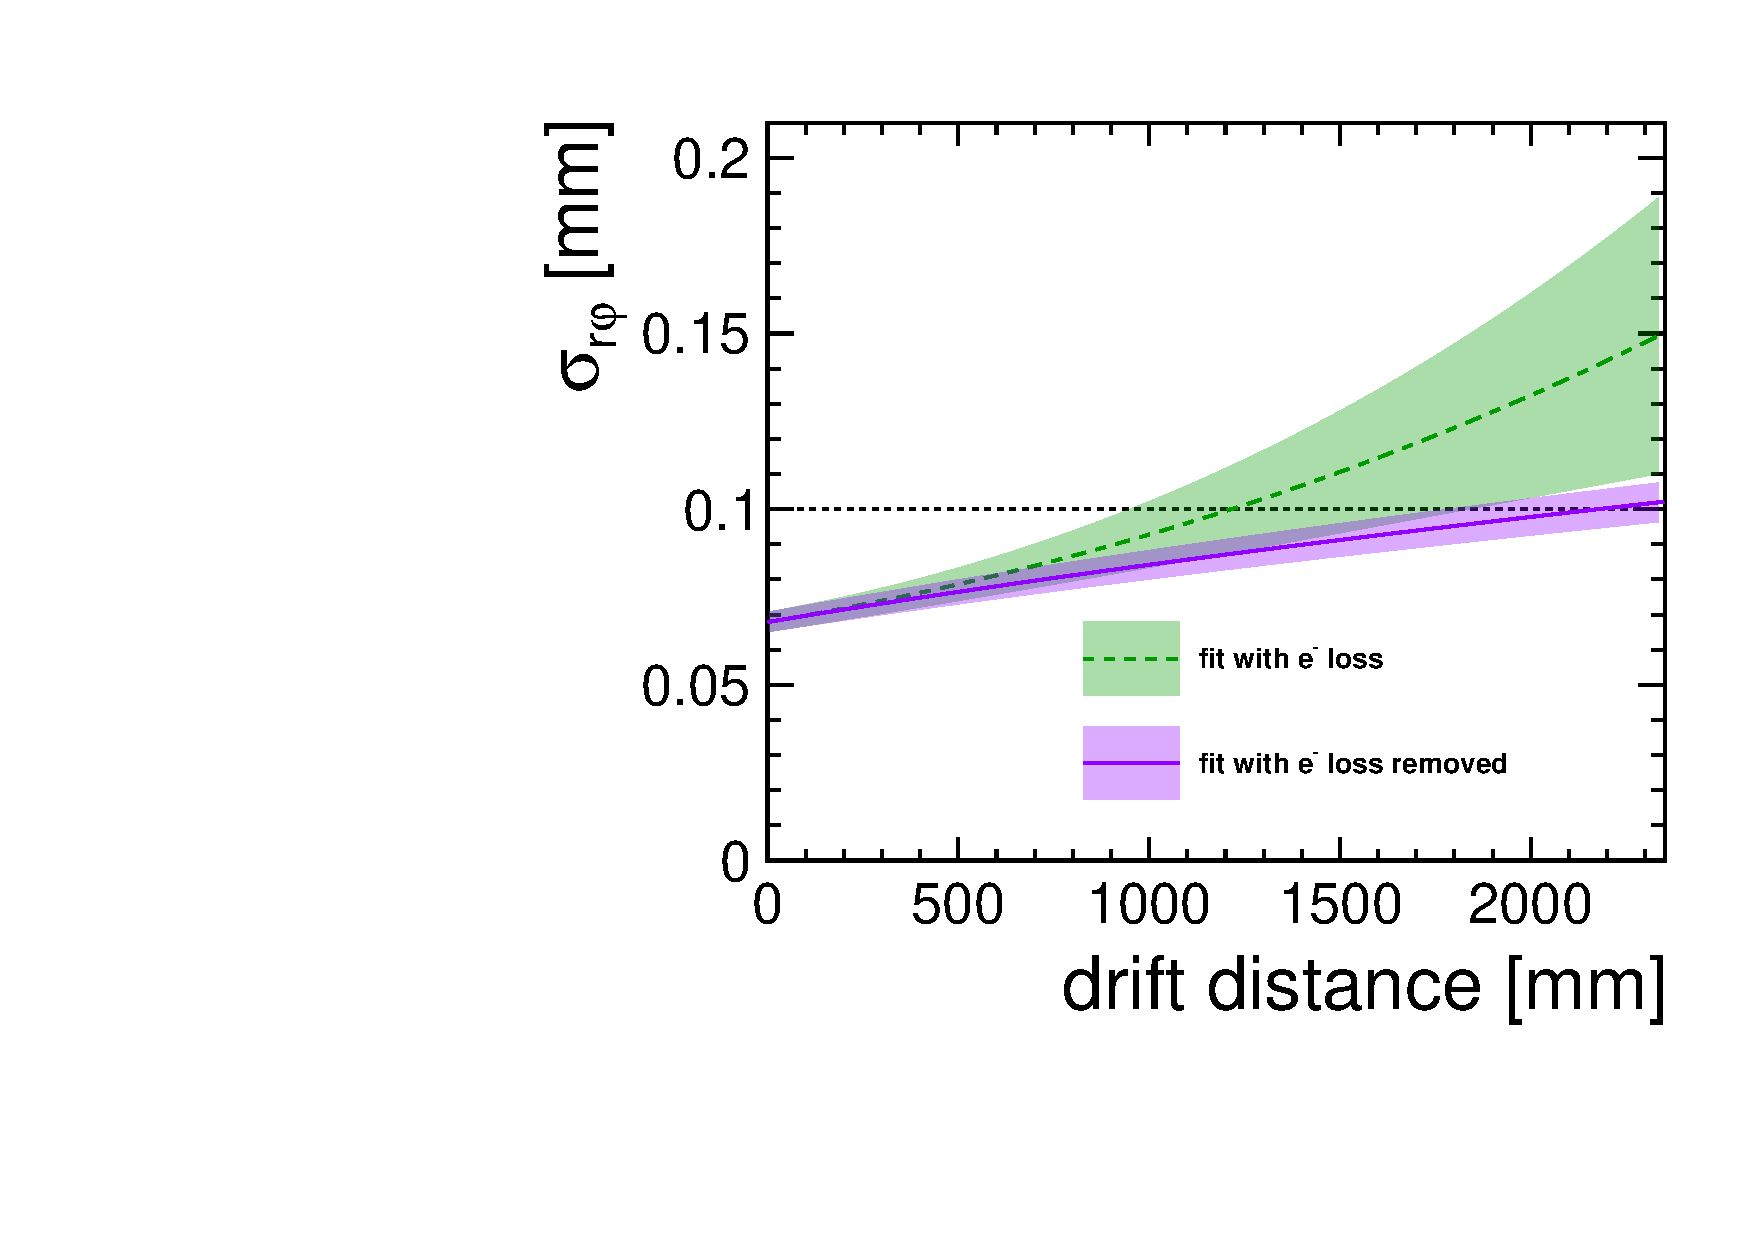
\includegraphics[height=0.4\textwidth]{Tracker/TPC_Bonn/plots/TPC-DG_resolutionExtrapolation2016_v2.pdf}
    \caption{Point resolution: extrapolation to a magnetic field of \SI{3.5}{T} based on parameters measured with the Large TPC Prototype at \SI{1.0}{T}. Plotted over the full ILD TPC drift length of \SI{2.35}{m} including 1 \sigma error bands. In red with the measured attachment rate, in green without any attachment.}
    \label{fig:resextrapol}
\end{figure}

In the 2016 beam test, several measurement runs were taken with so-called Minimal Ion Back Flow (MIBF) GEM-amplification settings, optimised to suppress ion back flow into the drift volume.
This goal is reached by limiting the amplification in the GEM facing the drift volume and optimising collection and extraction rates in the single GEMs by adjusting the electrical fields between them.
The detailed voltage settings and differences are shown in figure \ref{sfig:voltages_nom-mib}. 
The point resolution results of measurements runs with the adjusted amplification settings are shown in comparison to the standard point resolution in figure \ref{sfig:rphires_mibf}. 
It is visible that the impact of the adjusted amplification settings on the point resolution is close to negligible.

\begin{figure}
\begin{subfigure}[b]{0.52\textwidth}
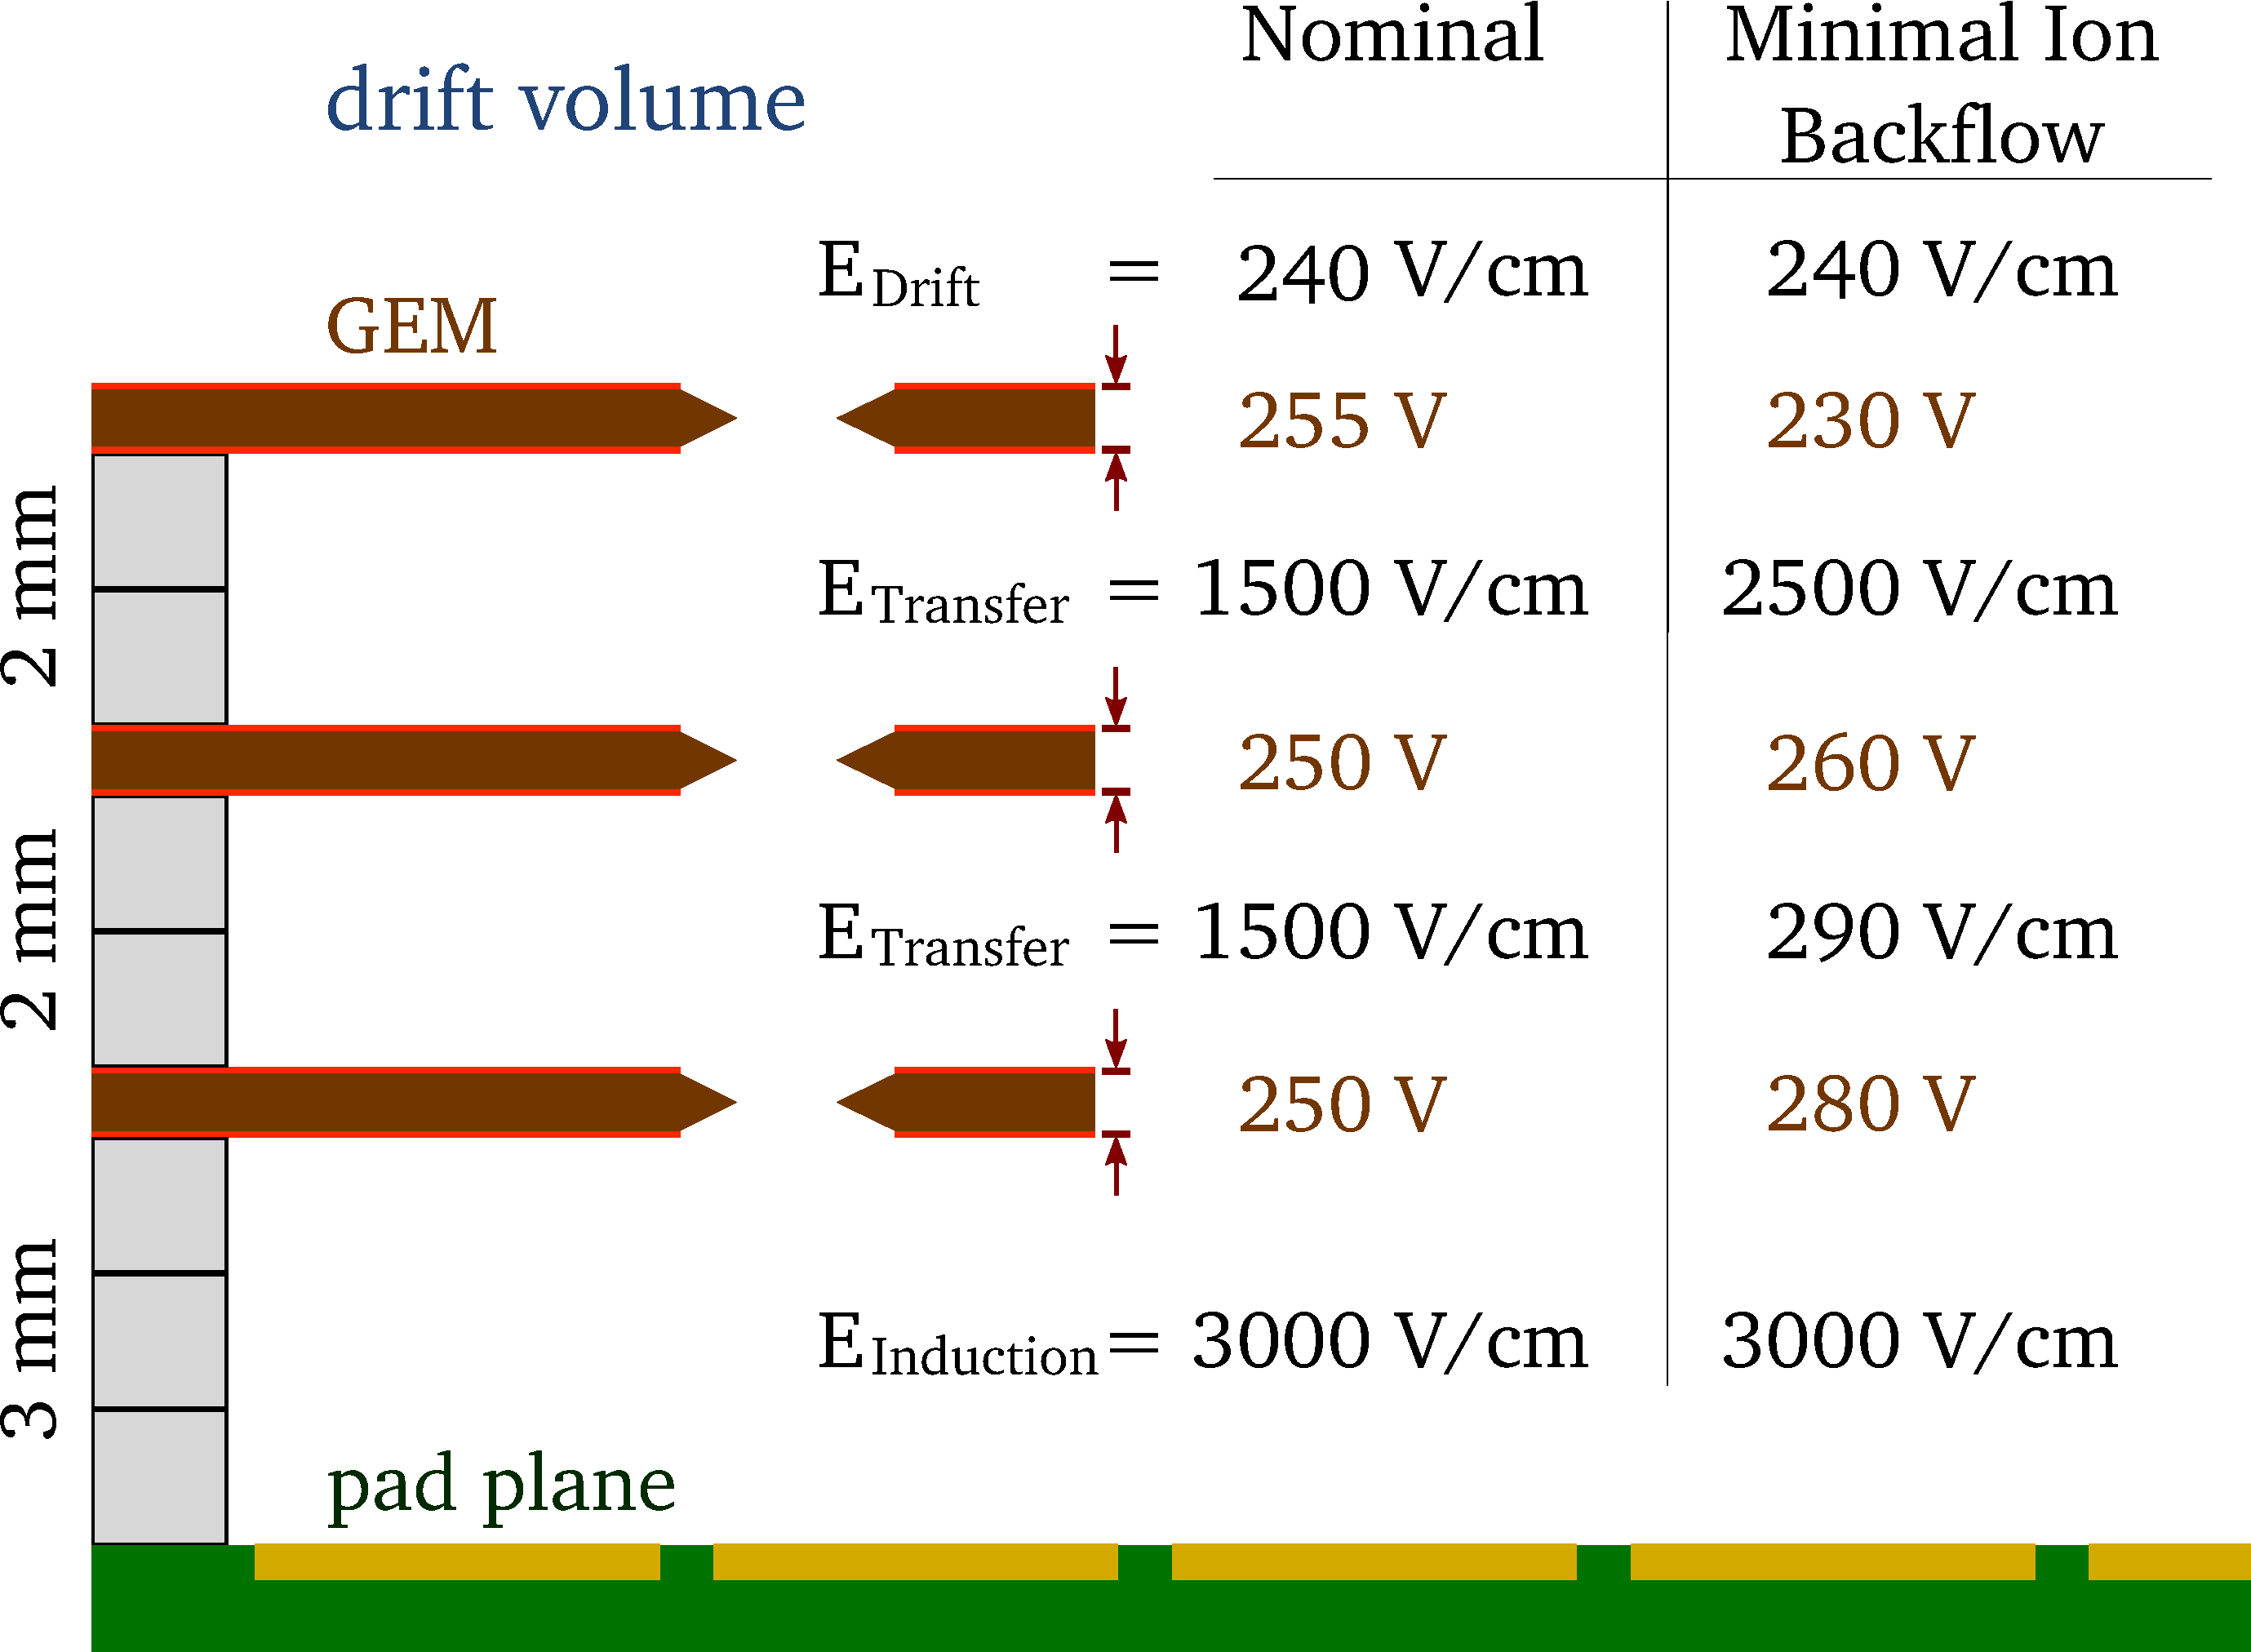
\includegraphics[width=\textwidth]{Tracker/TPC_Bonn/plots/TPC-DG_gem-voltages-nominal-mib.pdf}
\caption{Comparison of module voltages.}
\label{sfig:voltages_nom-mib}
\end{subfigure}%
\begin{subfigure}[b]{0.48\textwidth}
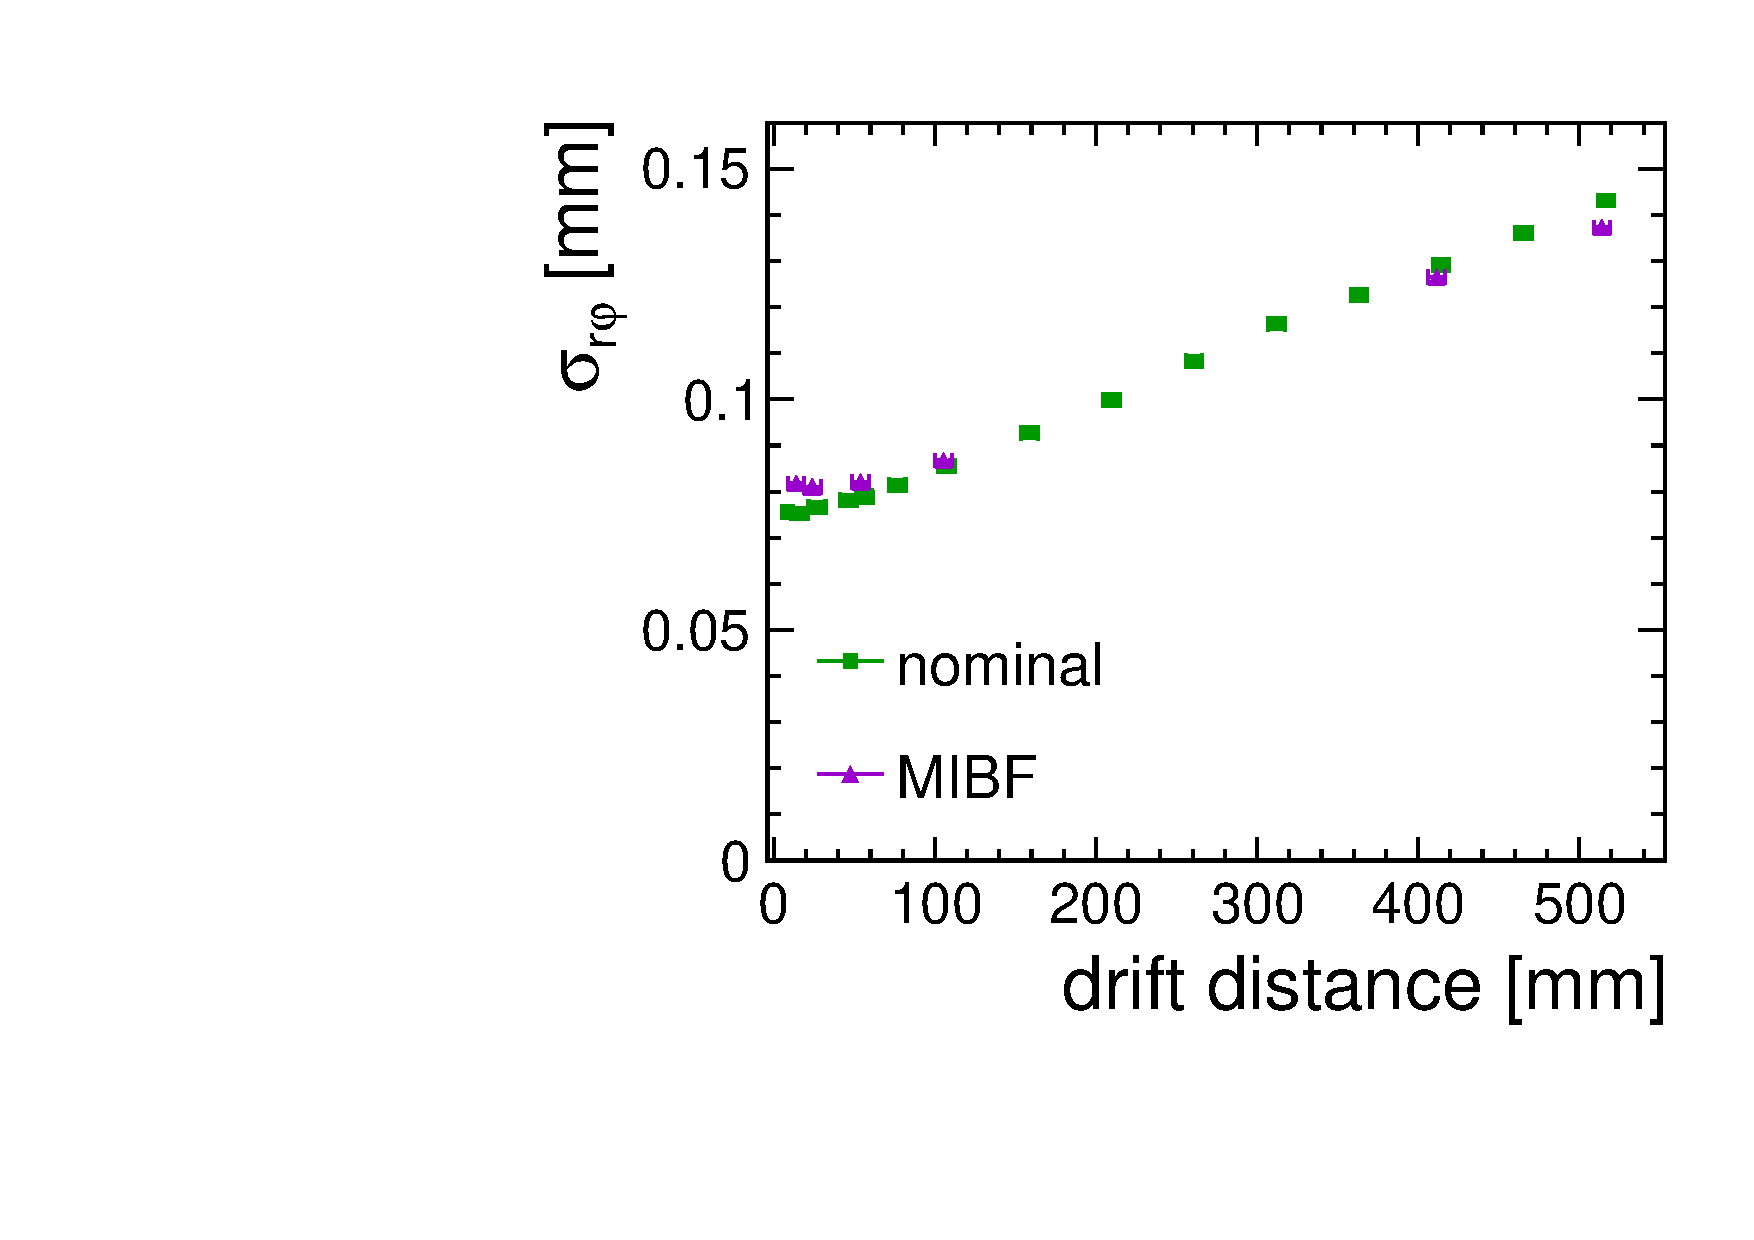
\includegraphics[width=\textwidth]{Tracker/TPC_Bonn/plots/TPC-DG_rphiResolution_IBF_v2.pdf}
\caption{Comparison of $r\varphi$\=/resolution.}
\label{sfig:rphires_mibf}
\end{subfigure}
\caption{Minimum ion backflow (MIBF):
  \protect\subref*{sfig:voltages_nom-mib})~The standard and the MIBF voltage settings in the GEM stack.
  \protect\subref*{sfig:rphires_mibf})~Comparison of the point resolution in $r\varphi$ for standard and MIBF settings.}
\label{fig:mibf}
\end{figure}

\paragraph{Double-Hit Separation}

To study the double hit separation capabilities of the system, a set of measurement runs has been performed with a steel target in front of the TPC prototype, see figure \ref{sfig:target_principle_simu}. 
Simulations showed that half a radiation length was the optimal target thickness and in this case about \SI{6}{\percent} of the events are suitable for this study.
They contain tracks that have overlapping charge depositions in the first two or more measurement rows where the beam enters the sensitive volume. 
Further, the contained tracks are well separated along more than \SI{40}{\percent} of the remaining rows towards the beam exit to allow for a reliable track reconstruction and extrapolation.

The data has been analysed using a triplet track finder and a simple hit splitting algorithm that searches for significant dips in the charge distribution in a pad row. 
In addition, a new combined track and hit finder based on a local road search with pad pulses has been implemented~\cite{Kleinwort:395416}. 

Double hit candidates identified using this new track finder can in addition be treated by a newly developed hit splitting algorithm that fits two pad response functions (PRF) to the charge signal.
The principle of this PRF fit is shown in figure~\ref{sfig:mergedhit}. 
The distinction if the hit in question is a single or double hit is taken based on several parameters as hit size and charge but also the $\chi^2$ of the fit functions.

\begin{figure}
\begin{subfigure}[b]{0.46\textwidth}
%\vspace{0.5cm}
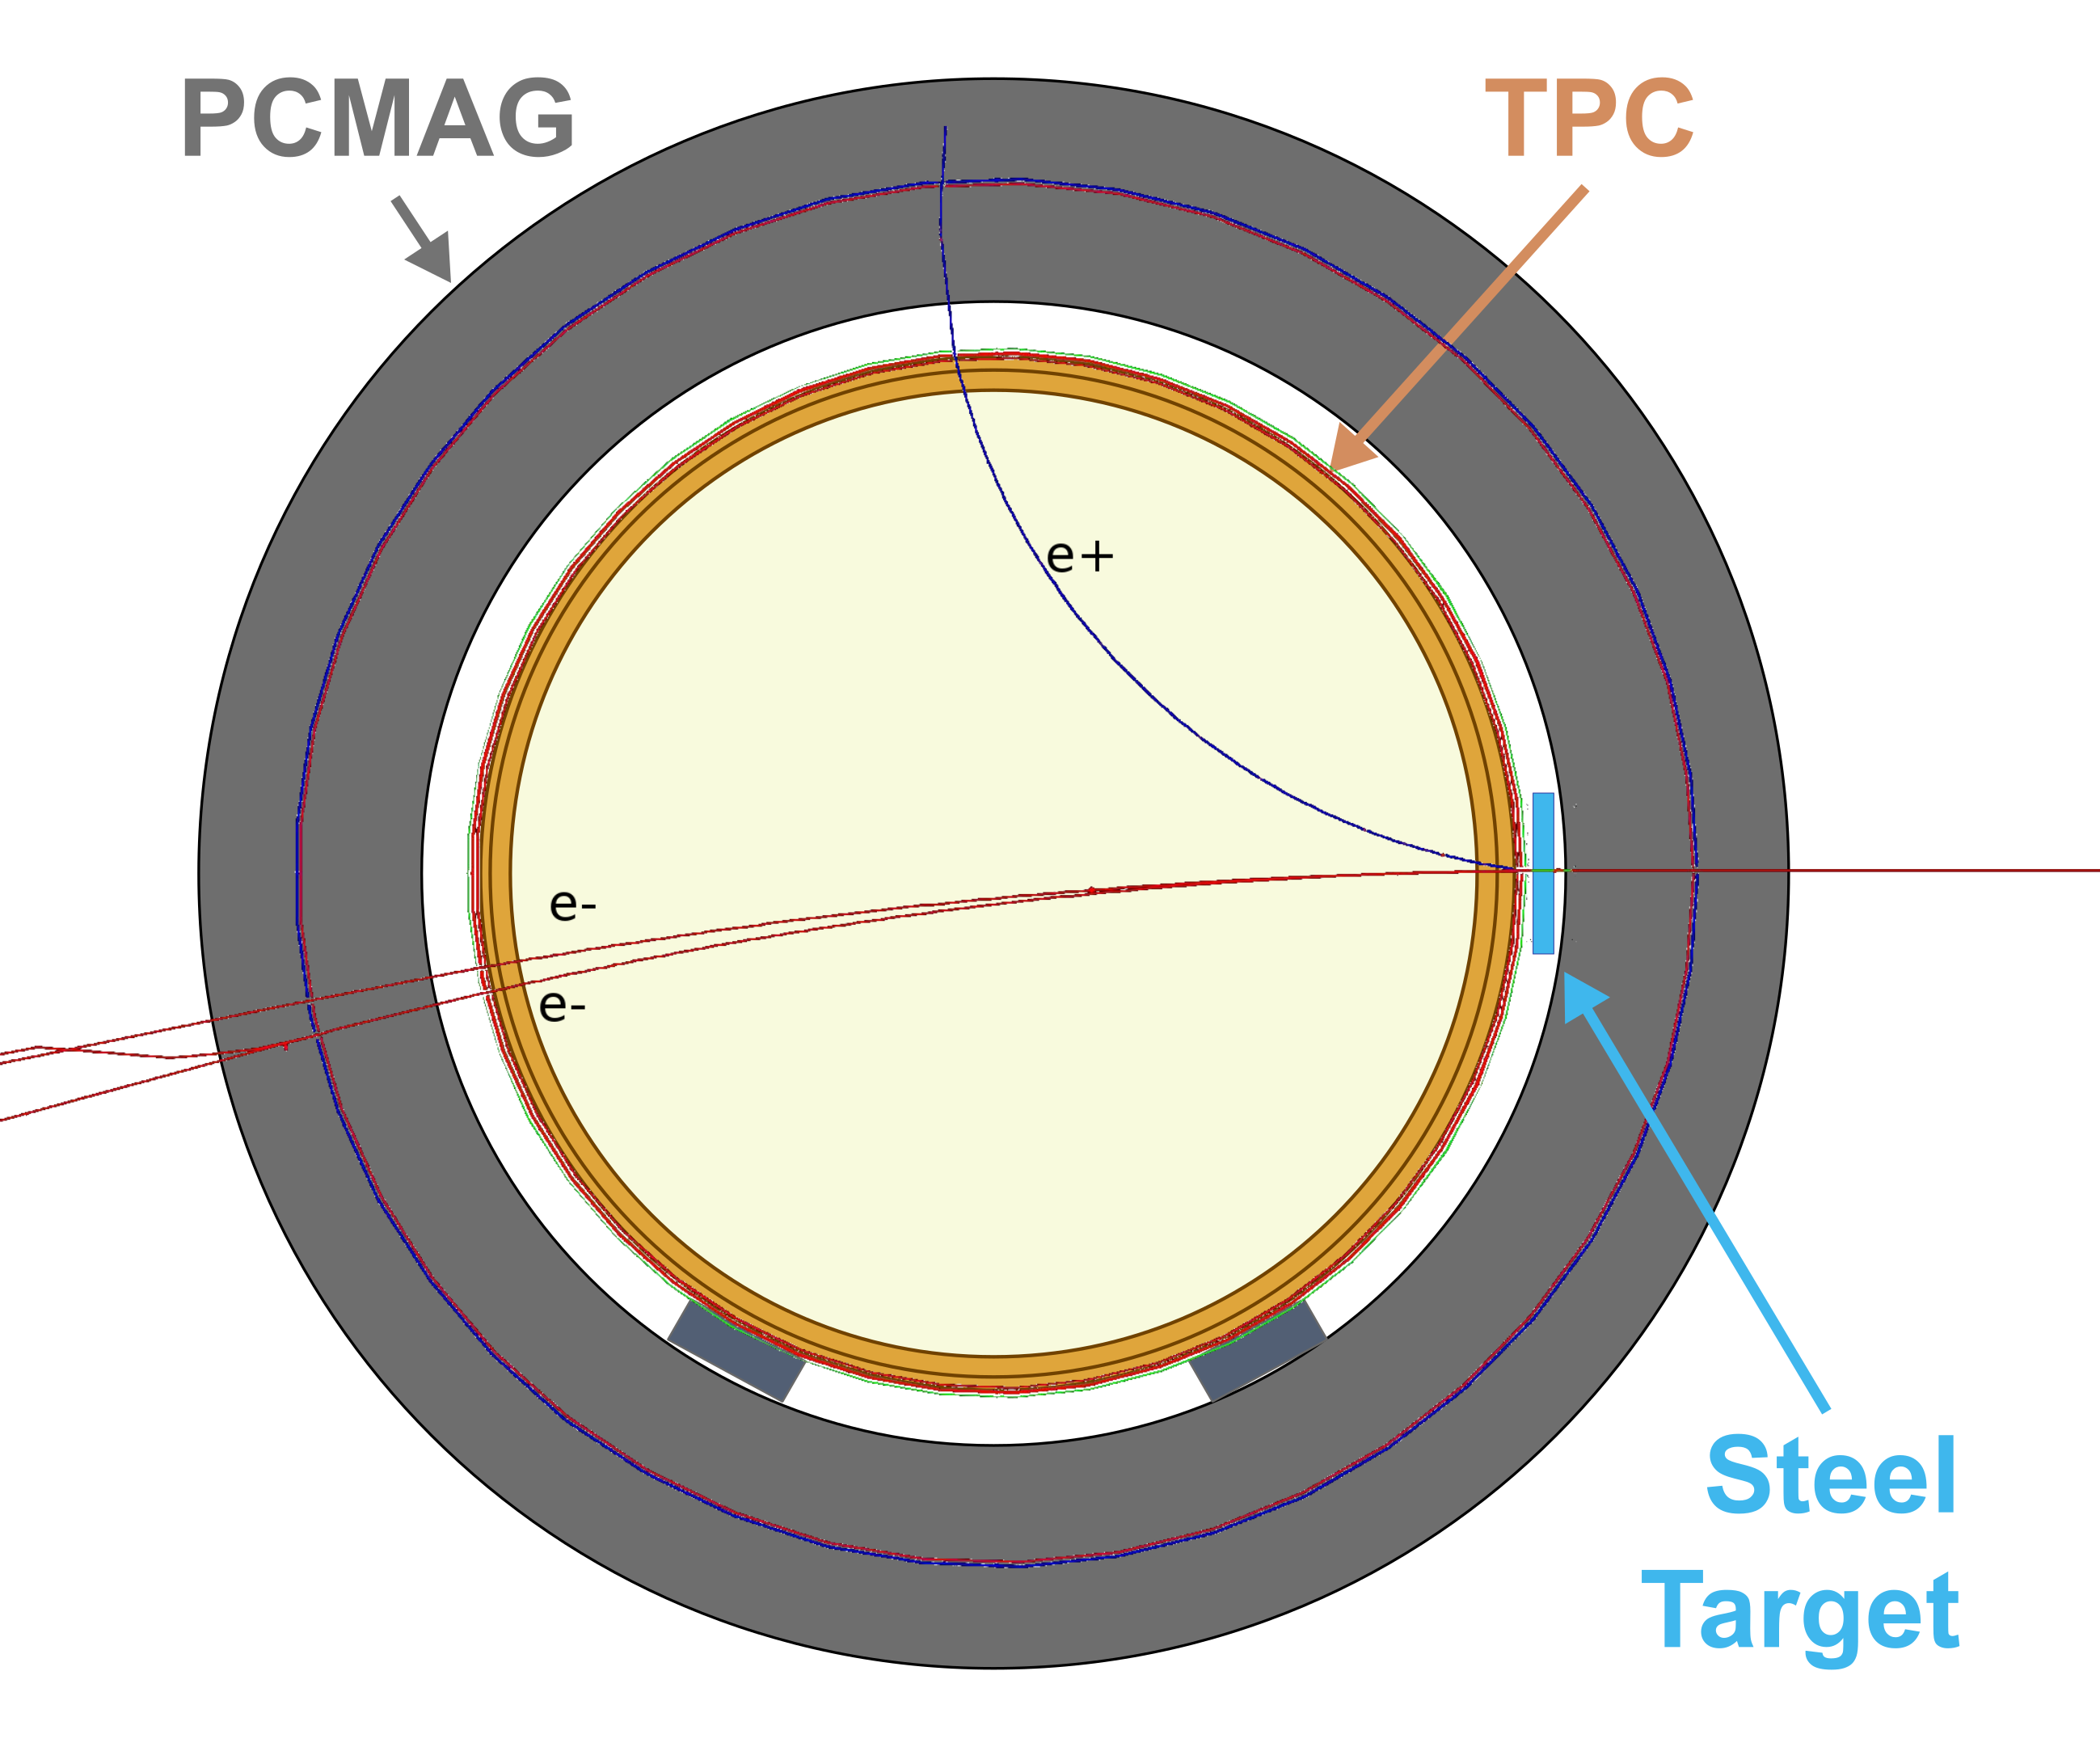
\includegraphics[width=\textwidth]{Tracker/TPC_Bonn/plots/TPC-DG_steel-target_principle_geant4.png}
\caption{Sketch of the target location.}
\label{sfig:target_principle_simu}
\end{subfigure}%
\begin{subfigure}[b]{0.54\textwidth}
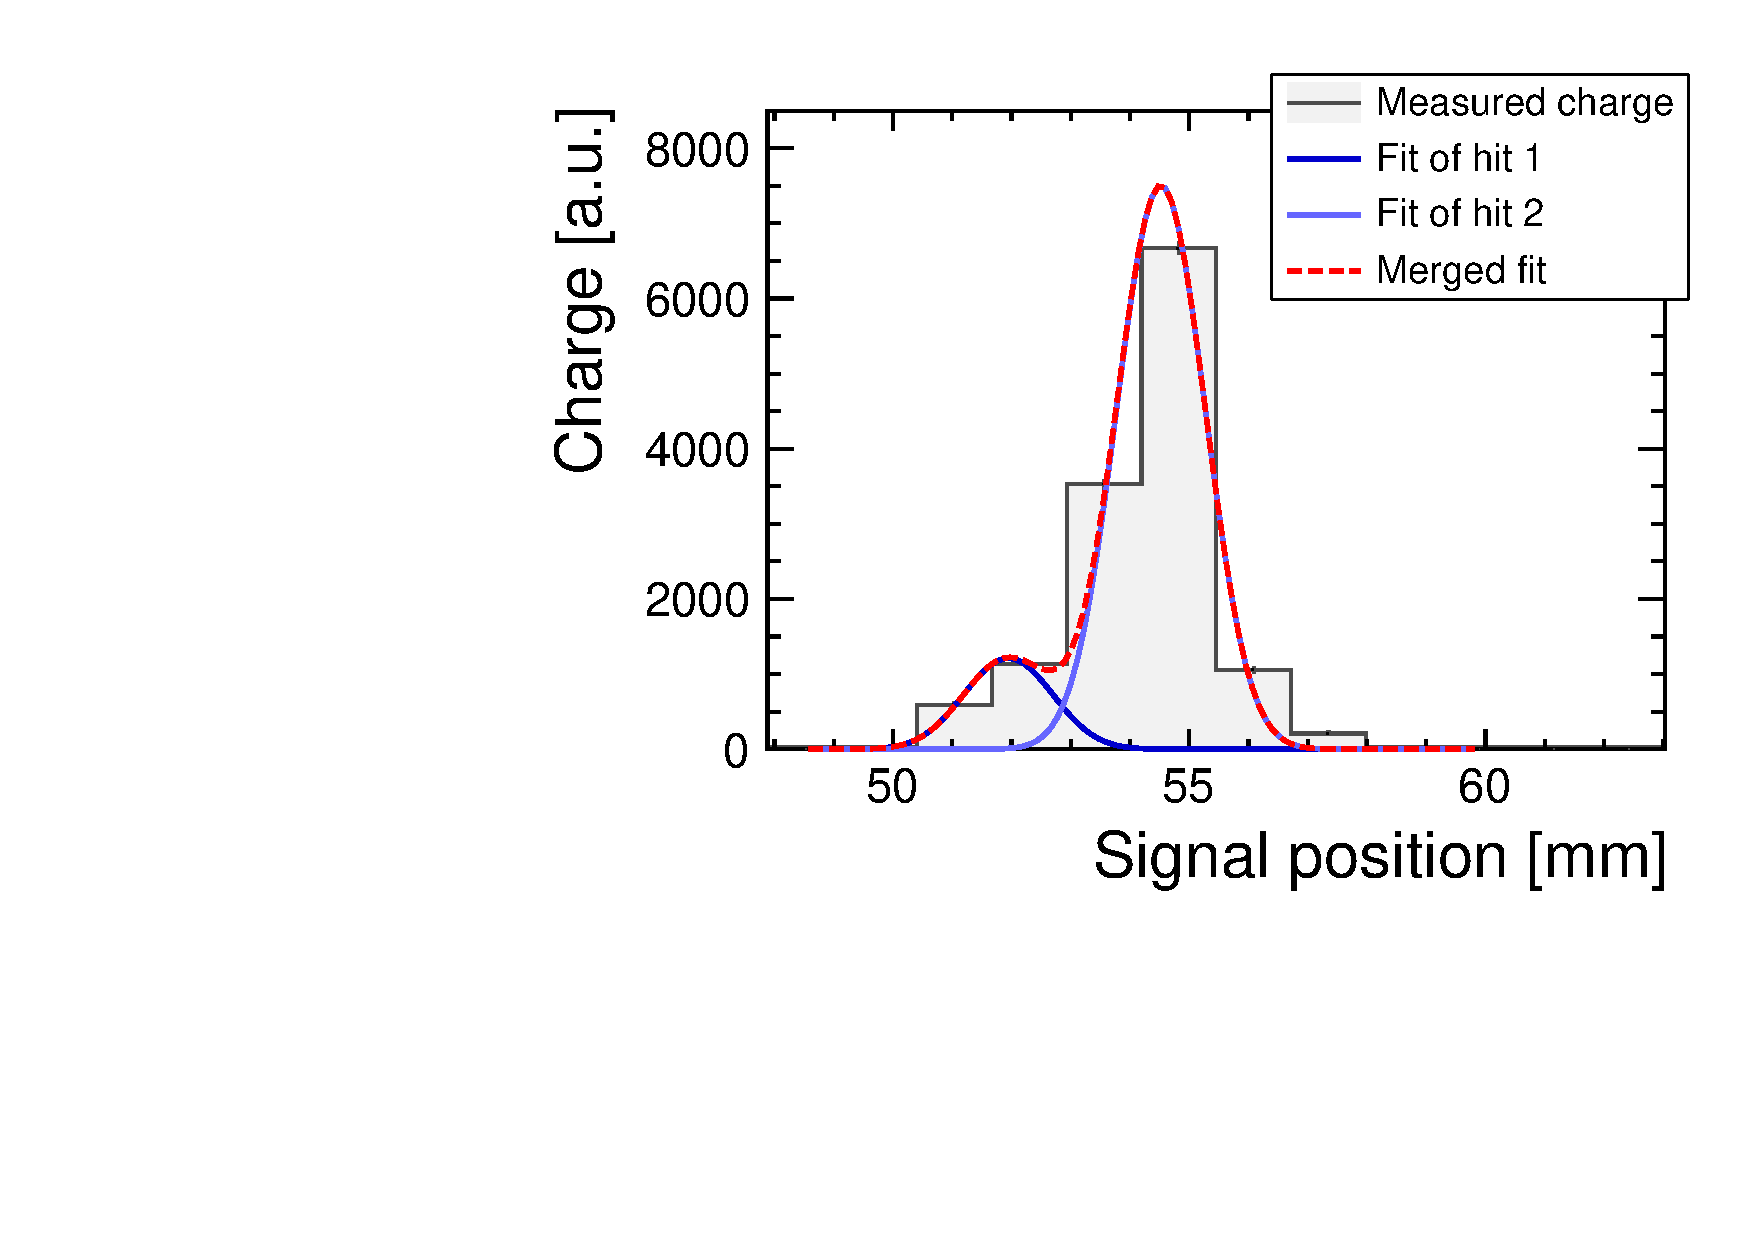
\includegraphics[width=\textwidth]{Tracker/TPC_Bonn/plots/TPC-DG_DoubleHitSplittingPrinciple.pdf}
\caption{Double-hit fitting.}
\label{sfig:mergedhit}
\end{subfigure}
\caption{\protect\subref*{sfig:target_principle_simu})~Sketch of the measurement setup for multi\-/track events, including an overlay of an event simulated with \textsc{Geant4}. \protect\subref*{sfig:mergedhit})~Schematic of the fit of the PRF (convolution of a box function and a Gaussian) to the signal of a merged double-hit.}
\label{fig:doublehitseparationprinciple}
\end{figure}

The traditional double hit separation has been compared to the results achieved with the combination of the two newly implemented approaches.
The results are shown in figure~\ref{fig:doublehitreso}. 
In figure~\ref{sfig:doublehitreso_data} it is clearly visible that the track distance down to which double hits can be split is improved by more than factor of two from about \SI{5}{\mm} down to about \SI{2}{\mm}. 
Figure~\ref{sfig:DHR_vs_drift_data} shows that the new approach improves the double hit separation similarly over all drift lengths.

\begin{figure}[tbhp!]
\begin{subfigure}[b]{0.5\textwidth}
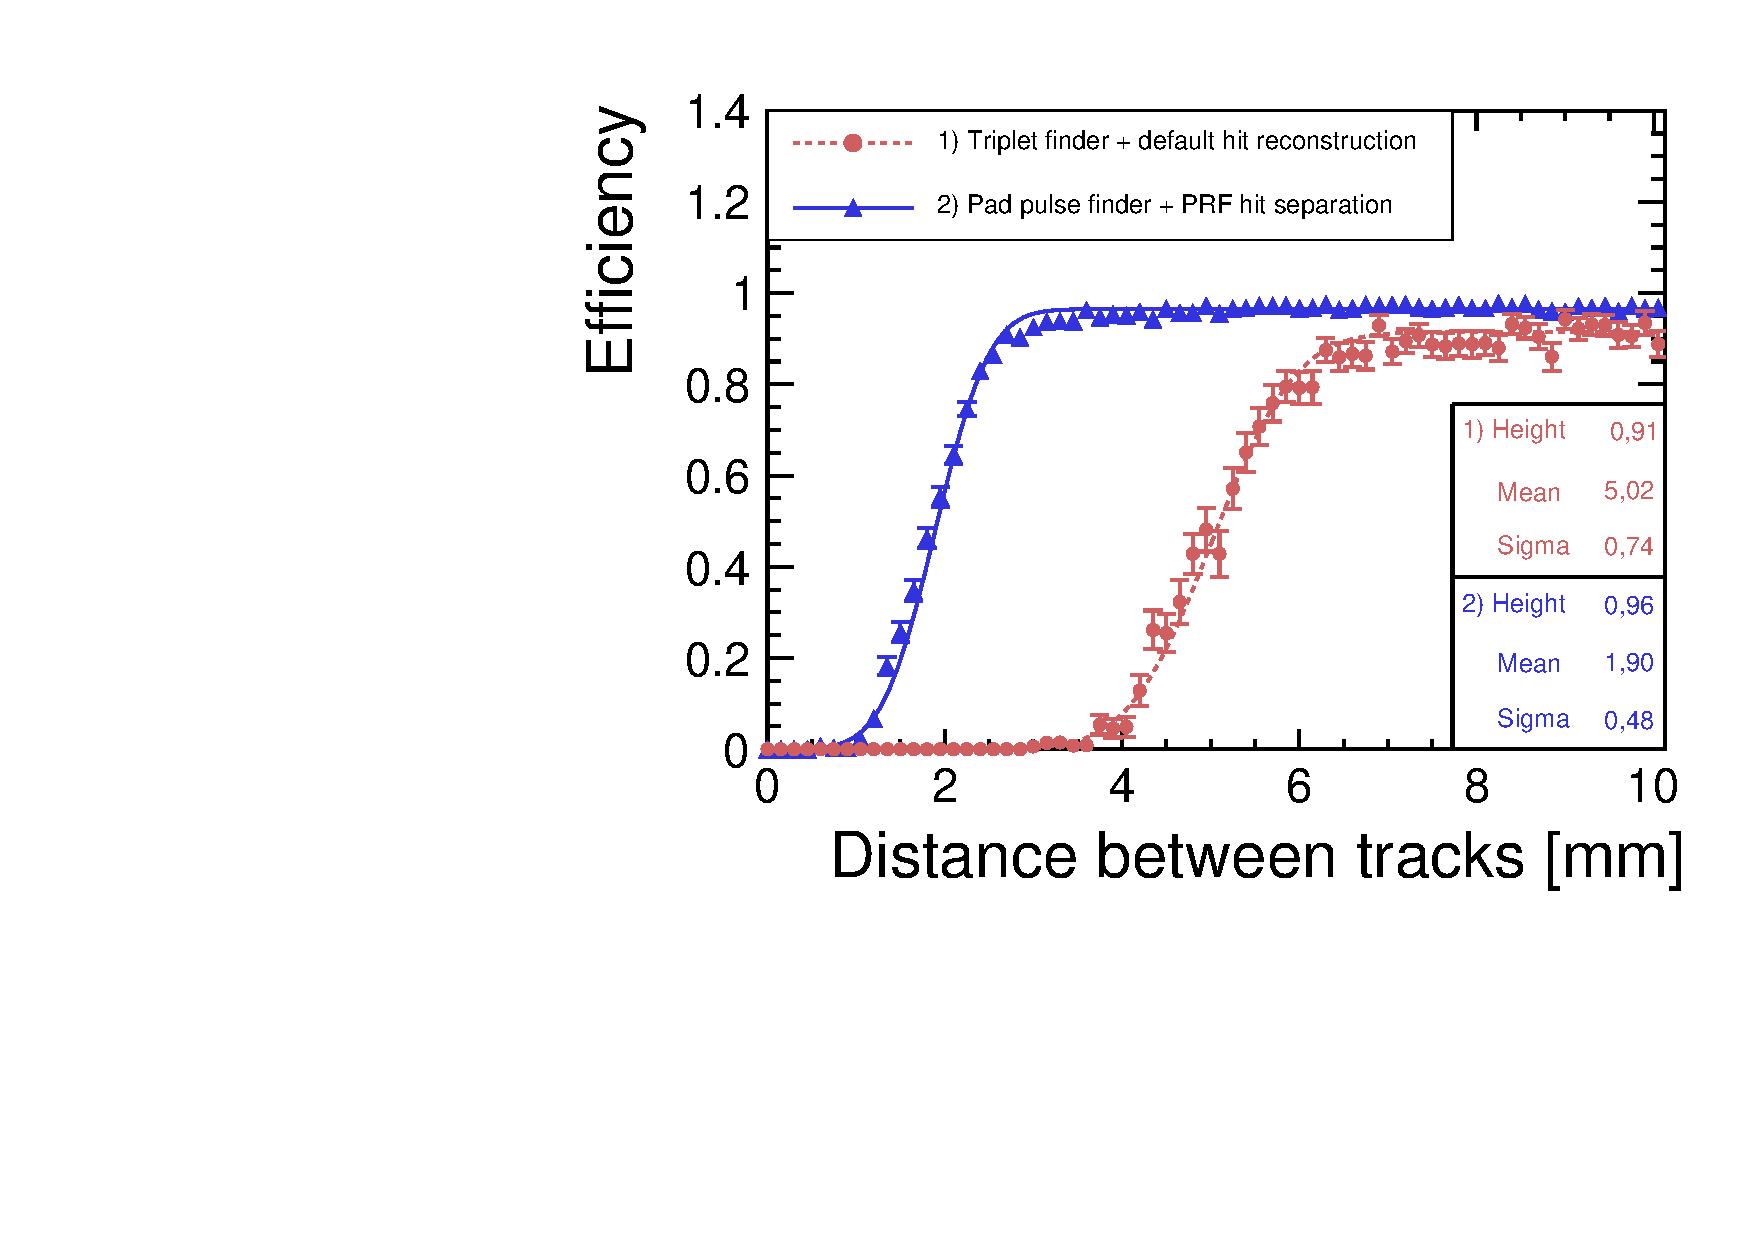
\includegraphics[width=\textwidth]{Tracker/TPC_Bonn/plots/TPC-DG_DHR_comp_Claus_Tripl_Bare2.pdf}
\caption{Measurement.}
\label{sfig:doublehitreso_data}
\end{subfigure}%
\begin{subfigure}[b]{0.5\textwidth}
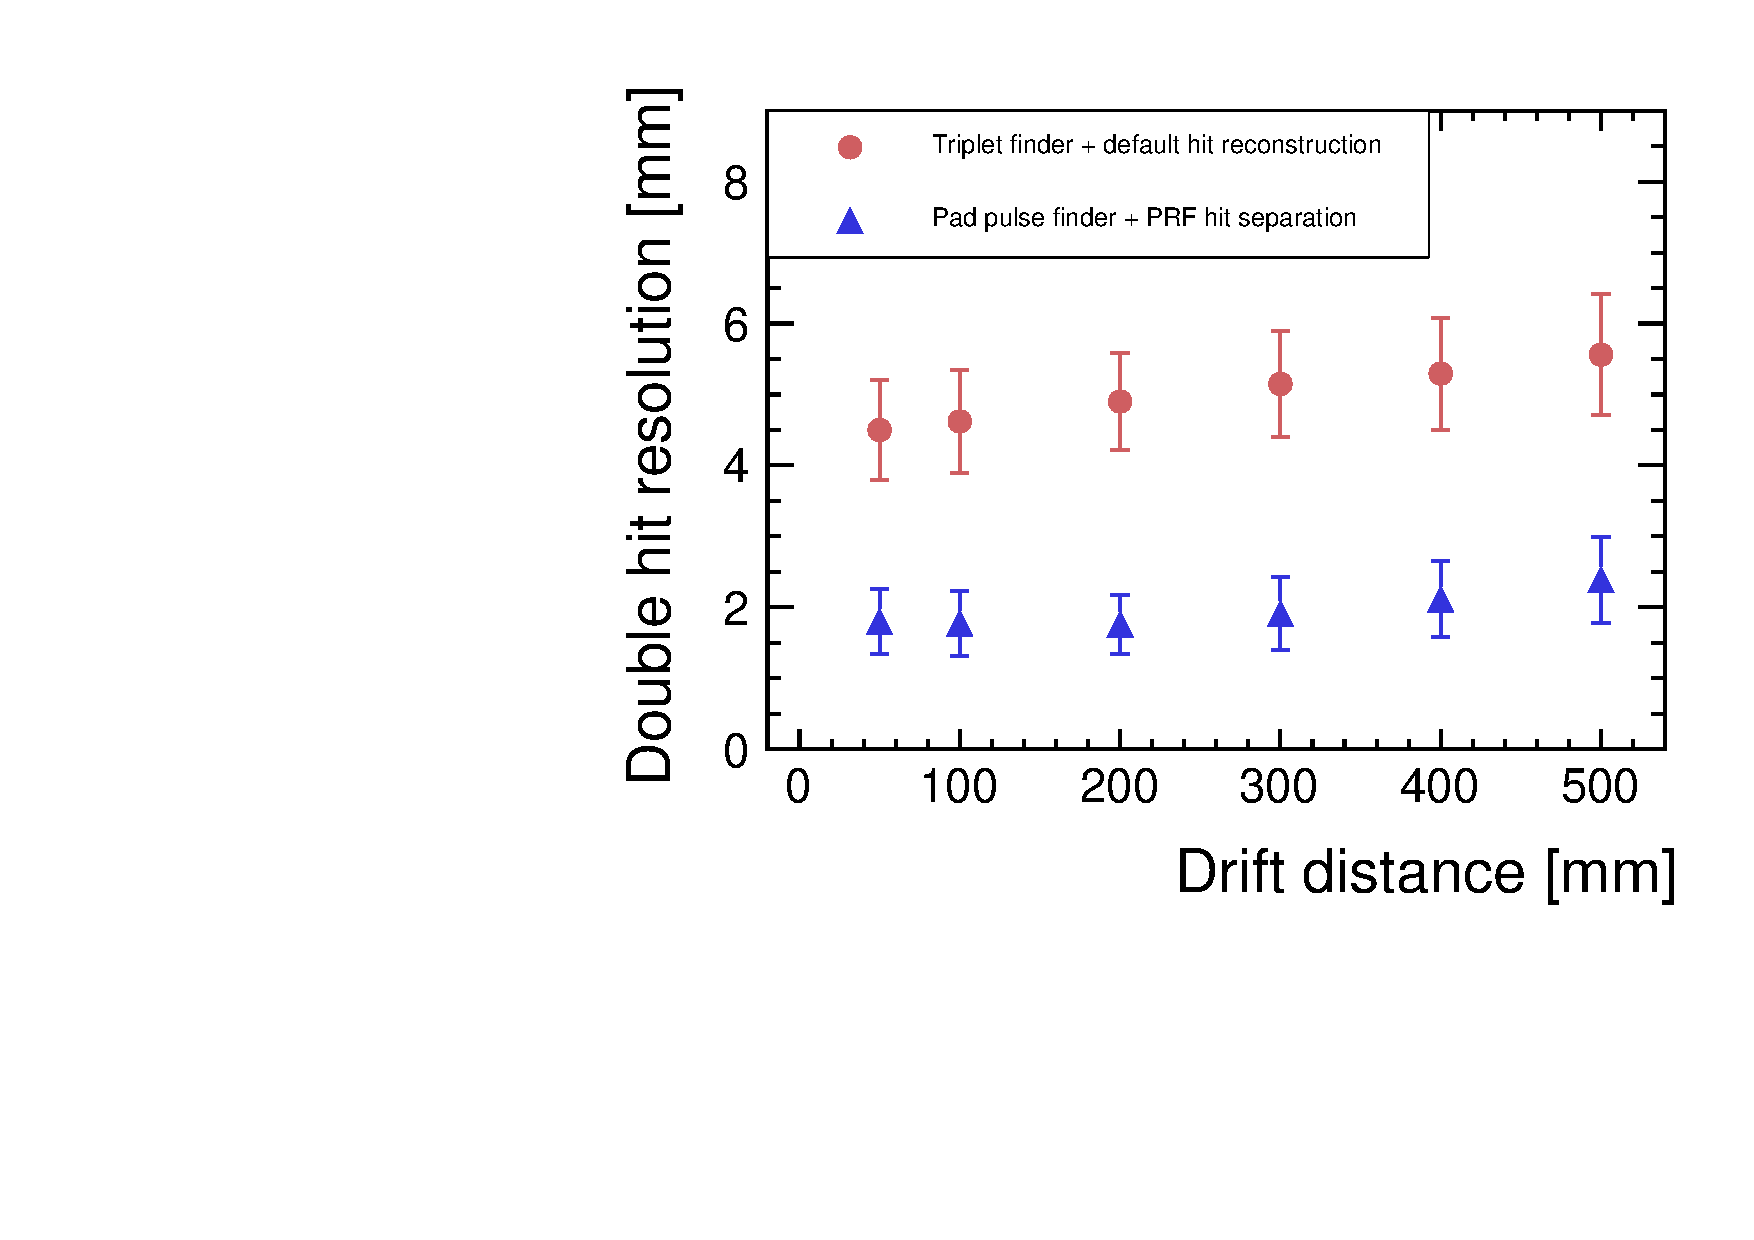
\includegraphics[width=\textwidth]{Tracker/TPC_Bonn/plots/TPC-DG_DHR_vs_drift_data.pdf}
\caption{Simulation.}
\label{sfig:DHR_vs_drift_data}
\end{subfigure}
\caption{\small Improvement of double-hit resolution: Shown are the results by using a standard triplet track finder without special merged hit treatment and of the pad pulse finder with additional PRF hit separation method. 
\protect\subref*{sfig:doublehitreso_data})~Comparison of the double-hit resolution.
\protect\subref*{sfig:DHR_vs_drift_data})~Double-hit resolution over the drift length. The bars depict the 1-$\mathrm{\sigma}$ range of the error function fitted in \protect\ref{sfig:doublehitreso_data} describing the efficiency in dependence of the track distance from zero to full separation.
}
\label{fig:doublehitreso}
\end{figure}

\paragraph{dE/dx Resolution}

The particle identification by measuring the specific energy loss \ensuremath{\mathrm{d}E/\mathrm{d}x} has been studied on the 2016 beam test data set. 
Certain quality criteria were applied to ensure an unbiased charge measurement for the \ensuremath{\mathrm{d}E/\mathrm{d}x} estimation.
Hits close to the module edges and GEM frames and hits containing one or more dead channels or double-hit candidates were excluded.
As estimator a truncated mean of \SI{75}{\percent} of the smallest samples is used, cutting off the tail towards high charge values visible in figure \ref{sfig:dedx_distr}.

For each track, the mean value of this truncated mean is used as the specific energy loss \ensuremath{\mathrm{d}E/\mathrm{d}x}.
The distribution from all tracks is plotted in \ref{sfig:dedx_mean} including a Gaussian fit in a range of three standard deviations around its mean value.
The relative \ensuremath{\mathrm{d}E/\mathrm{d}x} resolution is calculated from the RMS and mean of the distribution instead of the fit parameters.
This results in a \ensuremath{\mathrm{d}E/\mathrm{d}x} resolution of $\sigma_{\mathrm{d}E/\mathrm{d}x} = \SI[parse-numbers=false]{(8.95\pm0.02\pm0.14)}{\percent}$. 
Here, the first quoted error is the standard error of the weighted mean of its individual measurements.
The second quoted error reflects the standard deviation of the measurements, giving a systematic uncertainty.

\begin{figure}
\begin{subfigure}[b]{0.48\textwidth}
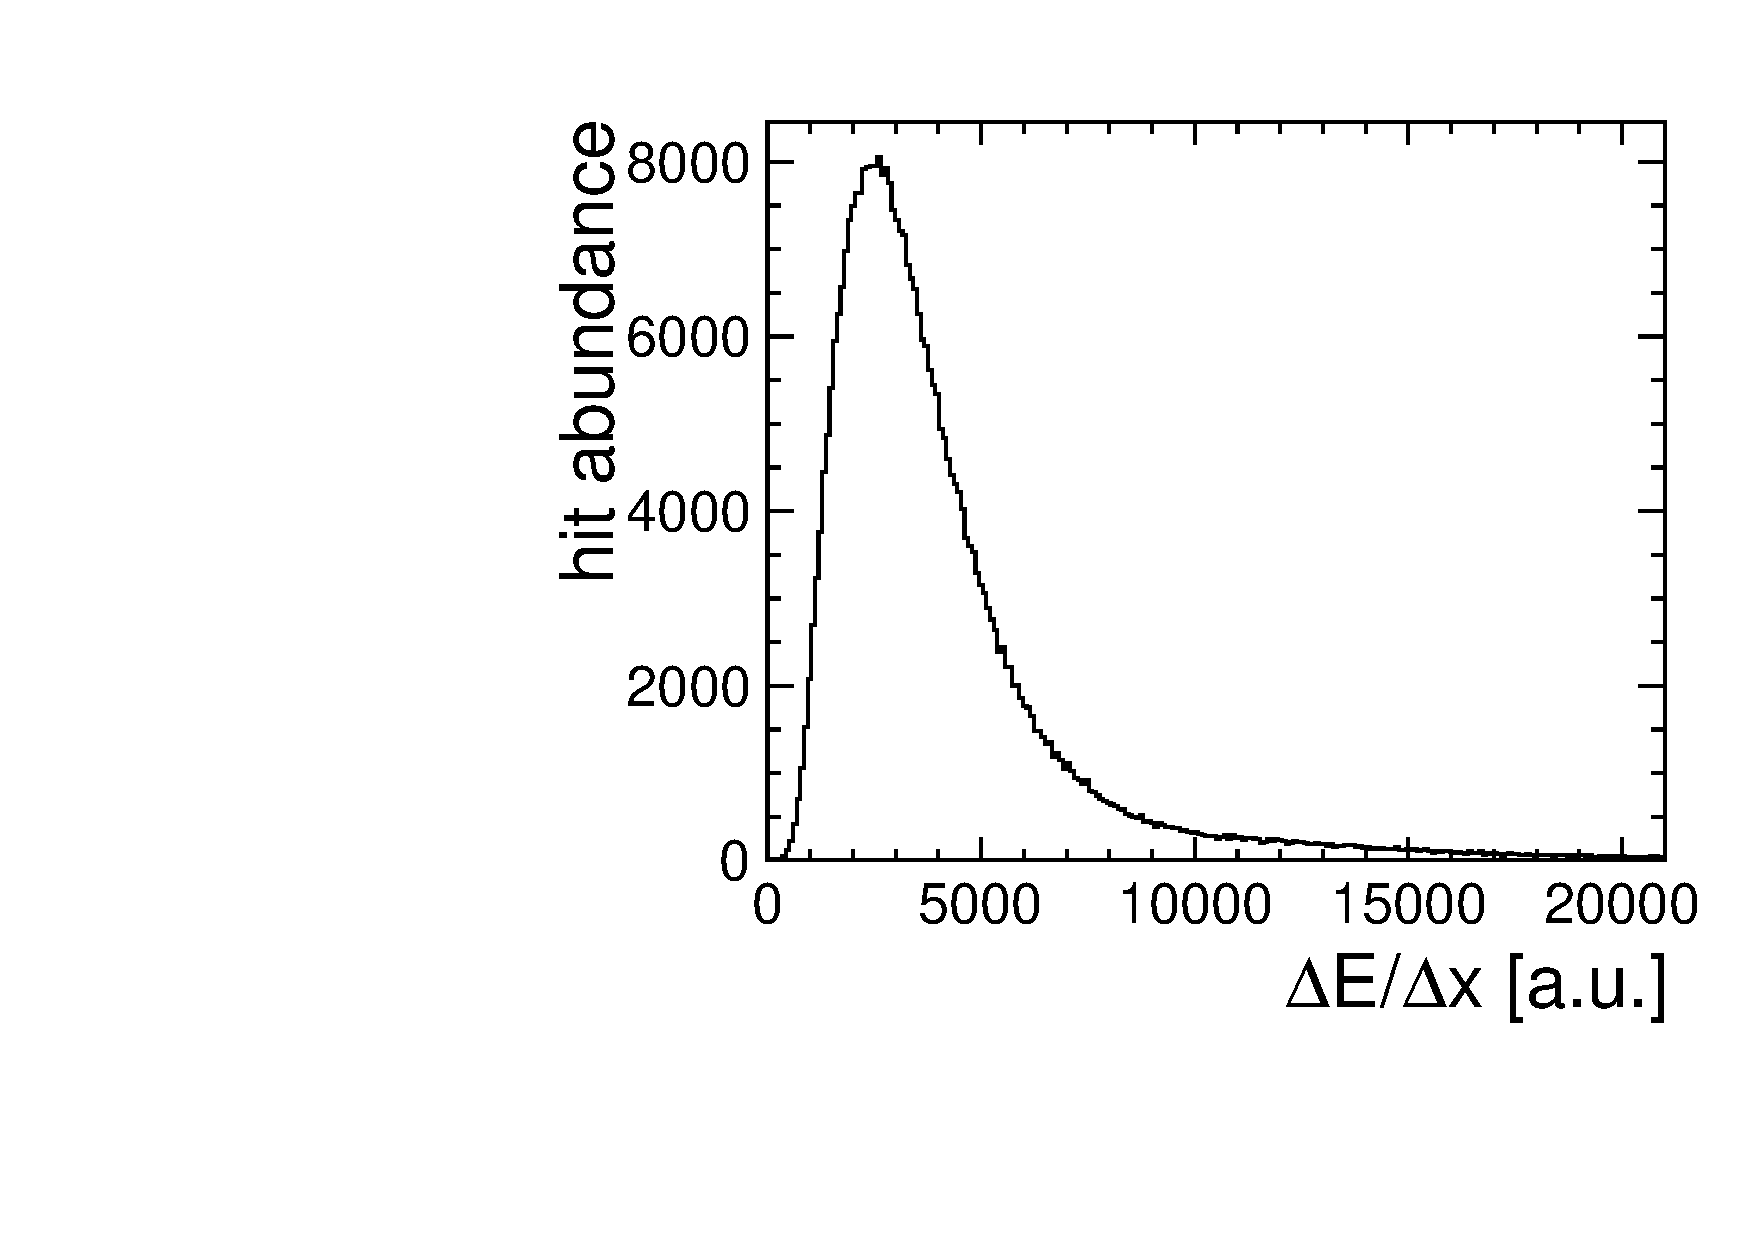
\includegraphics[width=\textwidth]{Tracker/TPC_Bonn/plots/TPC-DG_dEdxHitDist_v2.pdf}
\caption{}
\label{sfig:dedx_distr}
\end{subfigure}
\begin{subfigure}[b]{0.48\textwidth}
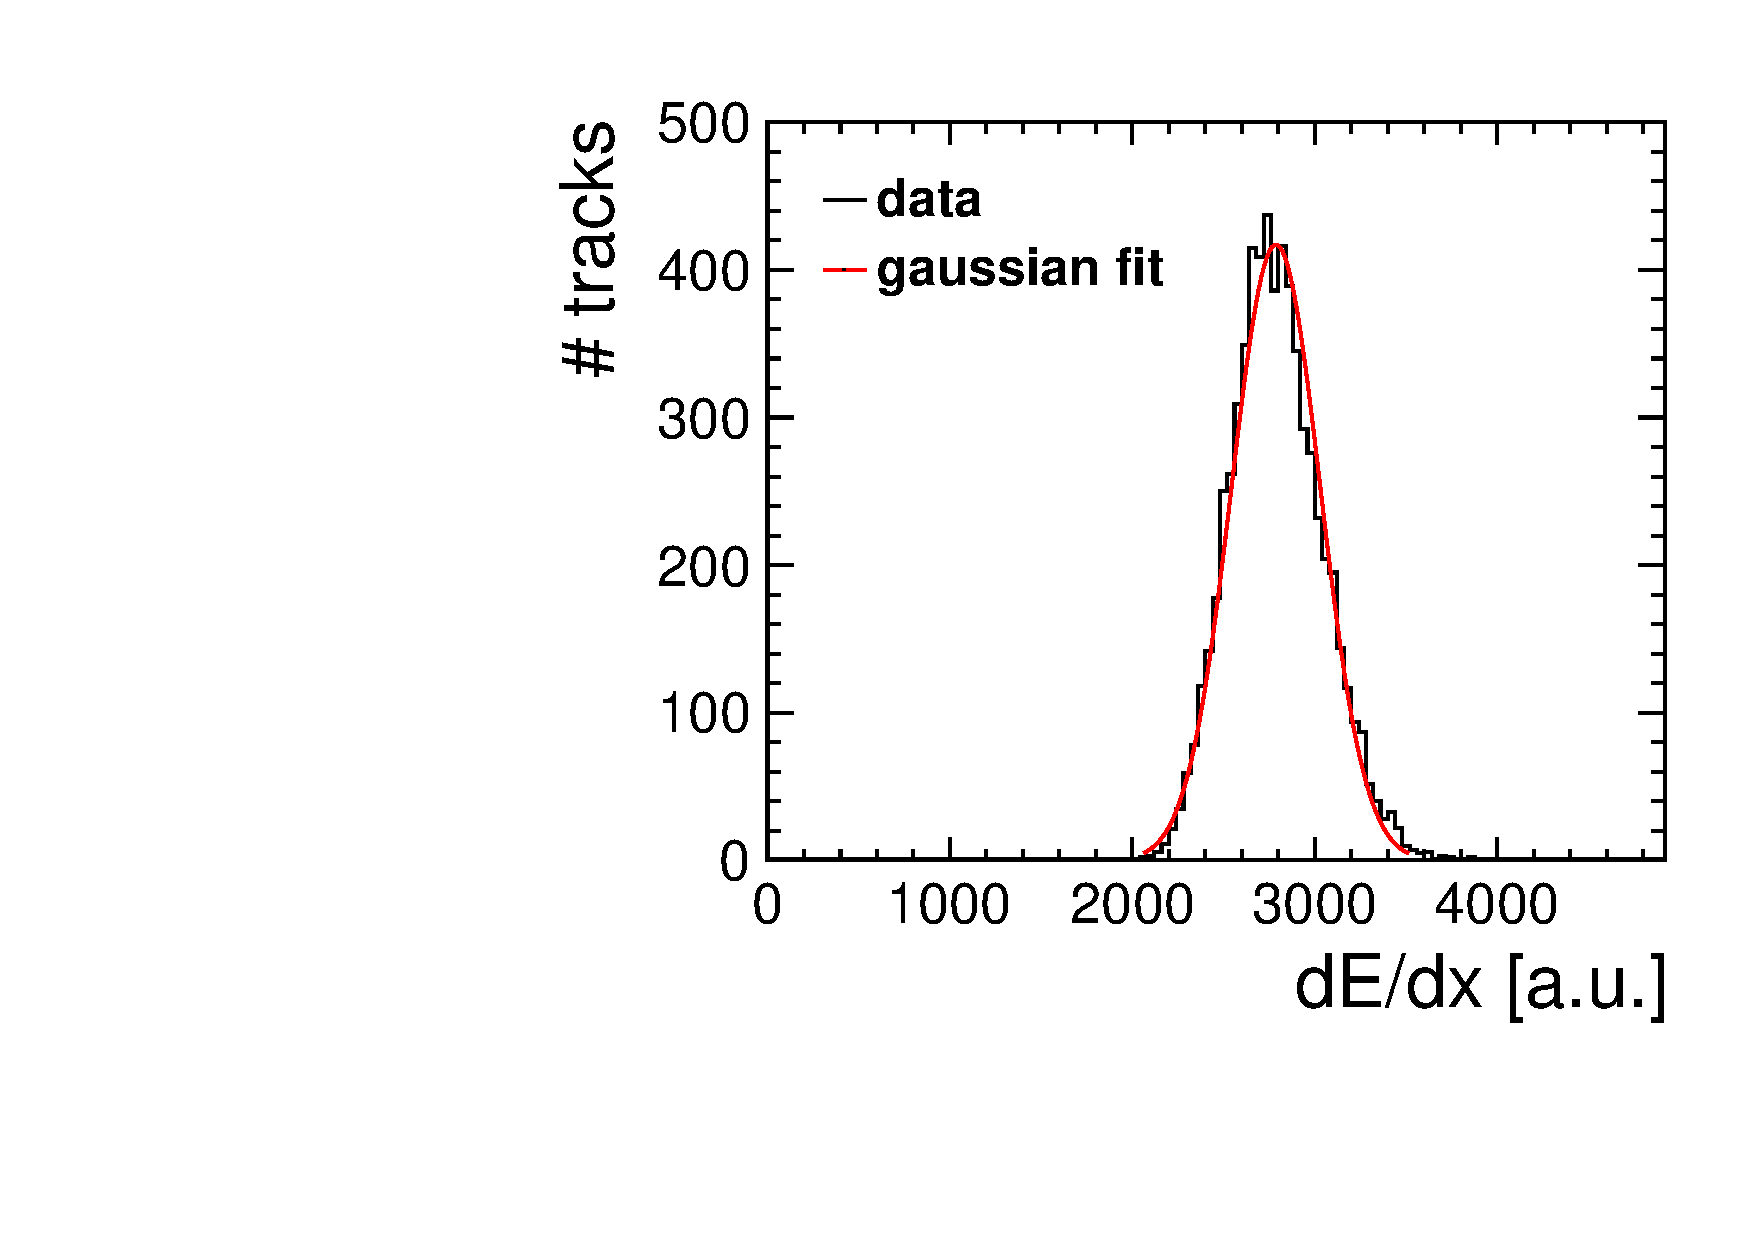
\includegraphics[width=\textwidth]{Tracker/TPC_Bonn/plots/TPC-DG_dEdxMeanDist_v2.pdf}
\caption{}
\label{sfig:dedx_mean}
\end{subfigure}
\caption{\small
  \protect\subref*{sfig:dedx_distr})~Distribution of the charge deposition per track length $\Delta E / \Delta x$ of a single track.
  \protect\subref*{sfig:dedx_mean})~Distribution of \ensuremath{\mathrm{d}E/\mathrm{d}x} for all tracks.
}
\label{fig:dedx_distributions}
\end{figure}

The achievable \ensuremath{\mathrm{d}E/\mathrm{d}x} resolution has also been extrapolated to the parameters of the final ILD TPC with \num{220} pad rows.
Here, a method relying exclusively on the beam test data is used combining hits from tracks in multiple events randomly.
Each hit is used only once to avoid correlations.
This allowed to create tracks from a few up to 220 hits.
The \ensuremath{\mathrm{d}E/\mathrm{d}x} resolution for the different track lengths is shown in figure \ref{sfig:dedx_reso_ILD}.
It is visible, that the resolution goal of \SI{5}{\percent} can be reached.

\begin{figure}
  \centering
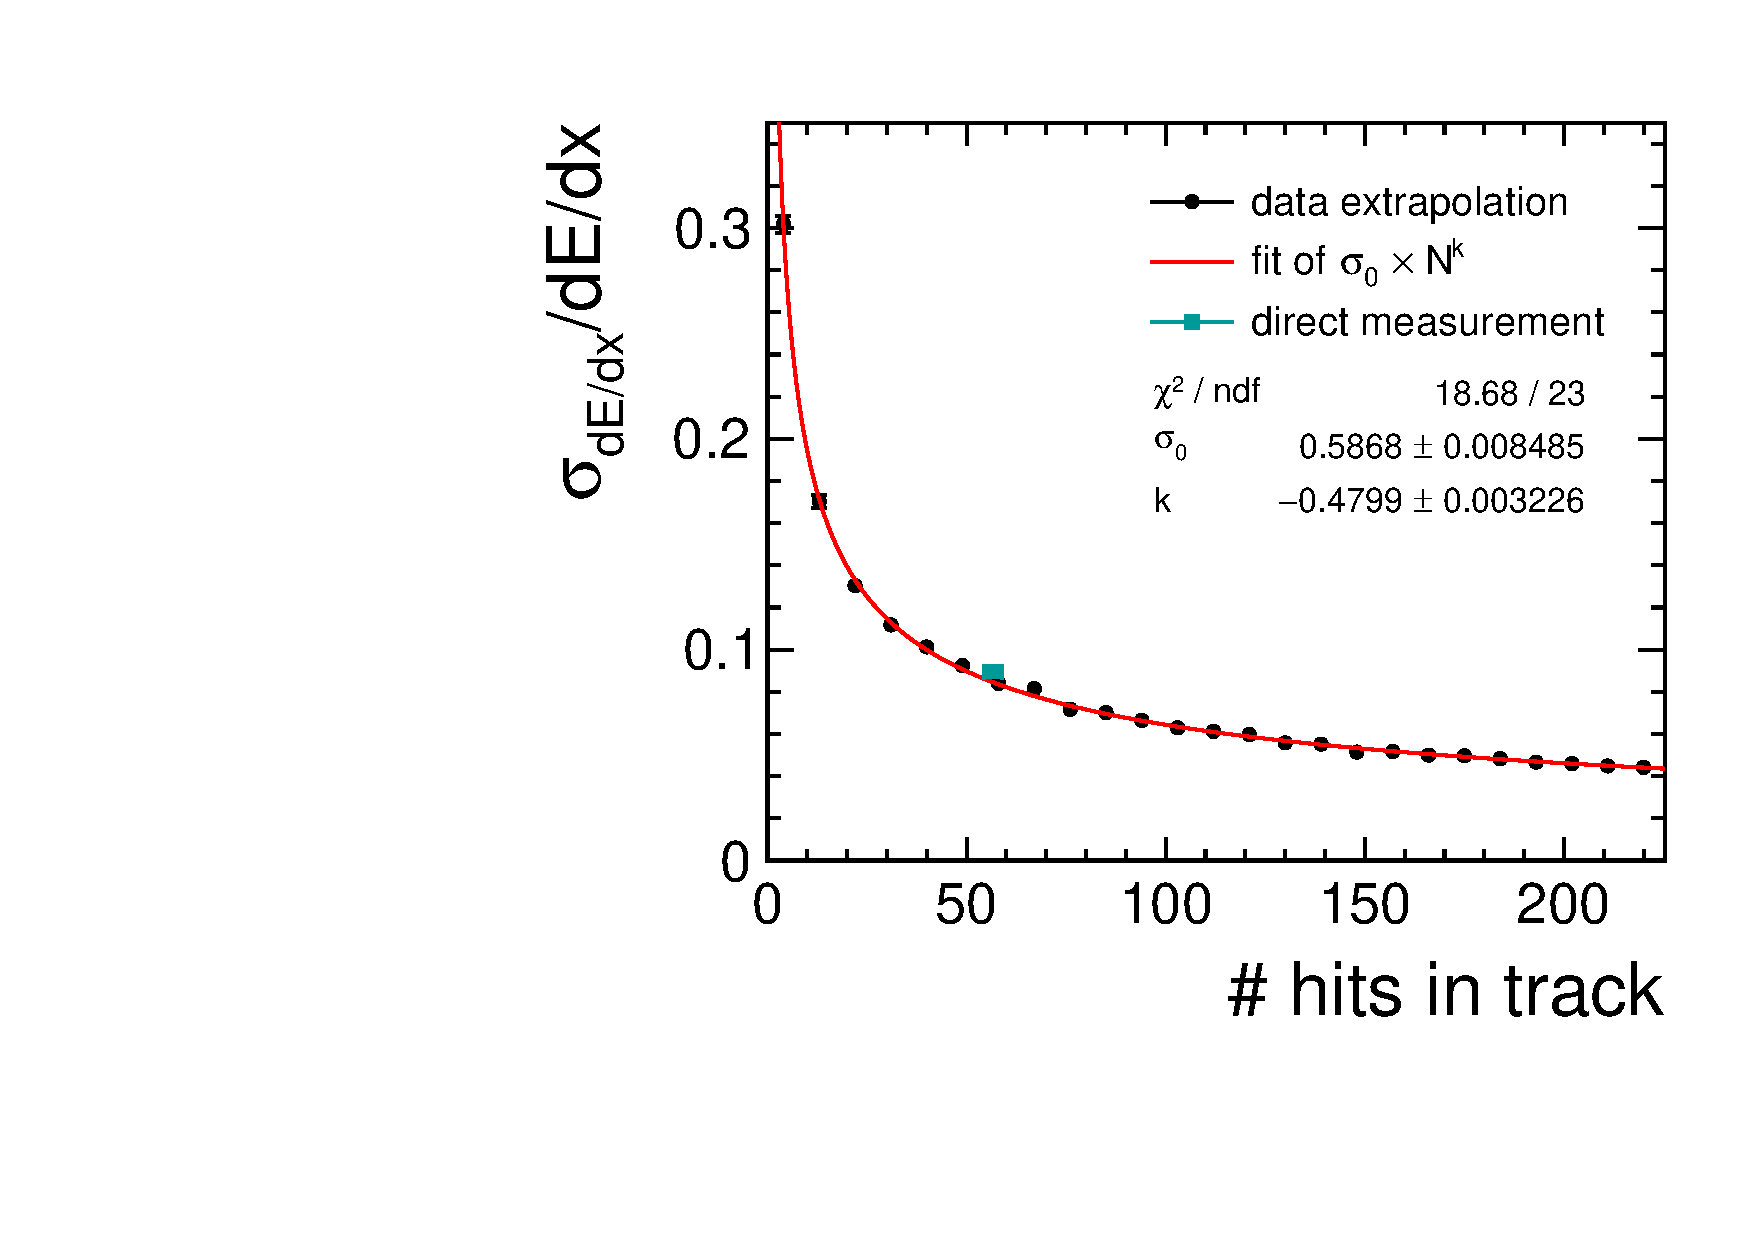
\includegraphics[width=0.5\textwidth]{Tracker/TPC_Bonn/plots/TPC-DG_dEdxResVSHits_fitPar.pdf}
\caption{Extrapolation, based on measured data,  of the \ensuremath{\mathrm{d}E/\mathrm{d}x} resolution to the ILD TPC.}
\label{fig:dedx_est}
\label{sfig:dedx_reso_ILD}
\end{figure}


\subsubsection{Future Plans}

By now three generations of these modules have been developed and successfully tested. The main issues which are going to be addressed in the next years are the
\begin{itemize}
\item re-optimization of the support structure for maximum mechanical strength and minimal interference with the readout.
\item optimization of the field-shaping integrated into the module, to minimize field distortions close to the module and at module boundaries.
\item integration of a GEM based gate on top of the current amplification structure, based on the recent developments at KEK.
\end{itemize}
The tooling developed to mount the GEM foil on the ceramic frames has been further improved since the last production. 
For the final module production, a mounting tool requiring less manual interaction leading to a faster and more automatized production will have to be developed.

\subsubsection{Engineering Challenges}
A detailed study is ongoing to understand and quantify the mechanical behavior of the ceramic frame GEM system. Bending tests have been performed, and compared to simulations. The interference between the mechanical properties and the electrical properties are studied. Measurements of the flatness of the module are being done, and will provide input for the next design iteration.
The fabrication of the ceramic frames which is currently done by laser cutting from solid sheets of ceramic will be studied. Possible alternatives are different production techniques and possibly material of the frames. Also, improvements in the laser cutting technology might allow thinner frames, without loosing stiffness.

Another open question is the distribution of the high voltage from the end plate to the different GEM layers. 
The current solution is rather labour intensive, and relies heavily on the skills of the person doing this connection. 
While with the third module generation the distribution system has been improved, it still relies on the same principle design as in the second version. 
Therefore, new solutions are being sought, which are easier to produce, more reliable, and will ensure reliably the high voltage stability. 
Connected to this protection schemes against accidental high voltage discharges are being further being studied and improved.

As discussed in section \ref{chap:TPC_sec:gating}, a gating GEM will be implemented as part of the amplification scheme. This gating GEM needs to be integrated mechanically and high-voltage wise into the module.

Currently a gap of about \SI{2}{mm} exists between neighboring modules. This gap introduces significant field distortions \cite{Zenker:2014qra}. They are partially compensated by a field shaping strip on the outside of each module. 
An improvement could be reached by further minimizing the gap between modules. Doing so will need improvements of the high voltage distribution, as discussed above, but also of the overall mechanical integration of the modules into the end plate. In addition, a more optimized design of the field shaping strip is planned. This has also to be incorporated in the design of the gating GEM mounting structure.
